%\documentclass{amsart}
\documentclass{article}

\usepackage{geometry}
\geometry{hmargin=2.5cm,vmargin=1.5cm}



% Fix "undefined control sequence \Everyshipout".
\usepackage{everyshi}

% Figures
\usepackage{dsfont}
\usepackage{graphicx}
\usepackage{subcaption}
\usepackage{float}
% \usepackage[justification=raggedright]{caption}	% makes captions ragged right - thanks to Bryce Lobdell
\usepackage{lscape}                                         % Useful for wide tables or figures.
\usepackage{wrapfig}
\usepackage[percent]{overpic}
\usepackage{tikz}

% Algorithm
\usepackage[lined,ruled,linesnumbered]{algorithm2e}
\usepackage{animate} %% convert frames to video

% Table and list
\usepackage{booktabs}                   % Publication quality tables
\usepackage{multirow}

\usepackage{makecell}

\usepackage{paralist}
\usepackage{enumitem}
\setlist[enumerate]{itemsep=0mm}

% Math
\usepackage{bm}                          % Make bold, italic math symbols
\usepackage{epsfig}                      % for figures
\usepackage{graphicx}                  % another package that works for figures
\usepackage{times}
% \usepackage{mathptmx}
\usepackage{mathtools}
\usepackage{amssymb,amsmath}   % Short math guide for LaTeX ftp://ftp.ams.org/pub/tex/doc/amsmath/short-math-guide.pdf

% Fonts
\usepackage{units}
\usepackage{color}

% Comments
\usepackage{comment}

% Hyperlinks
% \usepackage{url}  % Hyphenation of URLs.
%\usepackage[pagebackref=true,breaklinks=true,letterpaper=true,pagebackref=true,colorlinks,bookmarks=false]{hyperref}
\usepackage[pagebackref,breaklinks,colorlinks,linkcolor=blue,citecolor=blue,urlcolor=blue,bookmarks=false]{hyperref}
% \usepackage{authblk}
% \usepackage{slashbox}
\usepackage{xspace}
% \usepackage[table]{xcolor}
\usepackage{setspace}
\usepackage{grfext}
\PrependGraphicsExtensions*{.jpg,.png,.PNG}

\usepackage{gensymb}
% \usepackage{emoji}


% \usepackage{times,color}
% \usepackage{parskip}
% %\usepackage{epsfig}
% %\usepackage{psfig}
% %\usepackage[pdftex]{graphicx} % new acmsiggraph.cls
% \usepackage{ifthen}
% %\usepackage[draft]{hyperref} % new acmsiggraph.cls
% \usepackage{float}
% \usepackage{alltt}
% \usepackage{mathenv}
% \usepackage{amsmath}
% \usepackage{amssymb}
% \usepackage{amsthm}
% %\usepackage{rotating}
% \usepackage{newlfont} % for Box
% %\usepackage{ulem}
% \usepackage{floatflt}
% \usepackage{wrapfig}
% \usepackage{fixltx2e}
% \usepackage{subfig} % for subfloat
% \usepackage{multirow}
% \usepackage{cleveref}
% \usepackage{algorithmic}
% \usepackage{CJKutf8} % Chinese

\definecolor{purple}{rgb}{1, 0, 1}

\newcommand{\ie}{\emph{i.e.,}\xspace}
\newcommand{\eg}{\emph{e.g.,}\xspace}
\newcommand{\abr}{\emph{abbr.}\xspace}
\newcommand{\ea}{\emph{et al.}\xspace}
\newcommand{\gensync}{\emph{GenSync}\xspace}
\newcommand{\colosseum}{\emph{Colosseum}\xspace}
\newcommand{\srep}{\emph{SREP}\xspace} % Set Reconciliation Enhances
\newcommand{\srepsim}{\emph{SREPSim}\xspace}
% Propagation
\newcommand{\esrep}{\emph{E-SREP}\xspace}
\newcommand{\epsrep}{\emph{EP-SREP}\xspace}
\newcommand{\mesrep}{\emph{ME-SREP}\xspace}
\newcommand{\mempoolsync}{\emph{MempoolSync}}

\newcommand{\fref}[1]{Fig.~\ref{#1}}
\newcommand{\tref}[1]{Table~\ref{#1}}
\newcommand{\aref}[1]{Algorithm~\ref{#1}}
\newcommand{\procref}[1]{Procedure~\ref{#1}}
\newcommand{\sref}[1]{Section~\ref{#1}}
\newcommand{\lineref}[1]{line~\ref{#1}}
\newcommand{\appref}[1]{Appendix~\ref{#1}}

% Change \eqref
\LetLtxMacro{\originaleqref}{\eqref}
\renewcommand{\eqref}{Eq.~\originaleqref}

% Theorems and corollaries
\newcounter{theoremcount}
\setcounter{theoremcount}{0}
\DeclareRobustCommand{\theorem}[1]{%
  \refstepcounter{theoremcount}%
  \noindent\textit{\textbf{Theorem \thetheoremcount\label{theorem:#1}: }}%
}
\DeclareRobustCommand{\theoremref}[1]{Theorem~\ref{theorem:#1}}

\DeclareRobustCommand{\proof}{\emph{Proof:}\xspace}
\DeclareRobustCommand{\qqed}{\hfill$\blacksquare$}

\newcounter{corollcount}
\setcounter{corollcount}{0}
\DeclareRobustCommand{\coroll}[1]{%
  \refstepcounter{corollcount}%
  \noindent\textit{\textbf{Corollary \thecorollcount\label{coroll:#1}: }}%
}
\DeclareRobustCommand{\corollref}[1]{Corollary~\ref{coroll:#1}}

\newcounter{lemmacount}
\setcounter{lemmacount}{0}
\DeclareRobustCommand{\lemma}[1]{%
  \refstepcounter{lemmacount}%
  \noindent\textit{\textbf{Lemma \thelemmacount\label{lemma:#1}: }}%
}
\DeclareRobustCommand{\lemmaref}[1]{Lemma~\ref{lemma:#1}}

\newcounter{definitioncount}
\setcounter{definitioncount}{0}
\DeclareRobustCommand{\definition}[1]{%
  \refstepcounter{definitioncount}%
  \noindent\textit{\textbf{Definition \thedefinitioncount\label{definition:#1}: }}%
}
\DeclareRobustCommand{\defref}[1]{Definition~\ref{definition:#1}}

%notes of different authors
\newif\ifnotes
\notestrue
\notesfalse

\newif\ifdiff
\difftrue
\difffalse

\newcommand{\anote}[1]{\ifnotes $\ll$\textsf{\textcolor{purple}{Ari: {#1}}}$\gg$ \fi}
\newcommand{\nnote}[1]{\ifnotes $\ll$\textsf{\textcolor{orange}{Novak: {#1}}}$\gg$ \fi}
\newcommand{\diff}[1]{\ifdiff\textcolor{orange}{#1}\else#1\fi}

%%% Local Variables:
%%% mode: latex
%%% TeX-master: "main"
%%% End:

%\graphicspath{{figs/}} 
%%%%%%%%%%%%%%%%%%%%%%%%%%
\begin{document} 


\title{Improved Crouzeix-Raviart scheme for the Stokes and Navier-Stokes problem}
\author{E. Chénier, \footnote{ Univ Paris Est Creteil,  CNRS, UMR 8208, MSME, F-77454 Marne-la-Vallée, France \newline \texttt{eric.chenier@univ-eiffel.fr}}
\and 
E. Jamelot, \footnote{Universit\'e Paris-Saclay, CEA,  Service de Thermo-hydraulique et de M\'ecanique des Fluides, 91191 Gif-sur-Yvette, France \texttt{erell.jamelot@cea.fr}}
\and 
C. Le Potier, \footnote{Universit\'e Paris-Saclay, CEA,  Service de Thermo-hydraulique et de M\'ecanique des Fluides,  91191 Gif-sur-Yvette, France \texttt{christophe.le-potier@cea.fr}}
\and
A. Peitavy \footnote{Universit\'e Paris-Saclay, CEA, Service de Thermo-hydraulique et de M\'ecanique des Fluides, 91191 Gif-sur-Yvette, France \texttt{andrew.peitavy@cea.fr} }

} 


\newpage


\maketitle 

\begin{abstract}

The resolution of the incompressible Navier-Stokes equations is tricky, and it is well known that one of the major issue is to approach the space: $$ \bH^1(\Omega) \cap \bH(\dive0;\Omega):=\left\{\vvec\in \bH^1(\Omega)\, :\, \dive\vvec = 0 \right\}. $$ 
The non-conforming Crouzeix-Raviart finite element are convenient since they induce local mass conservation. Moreover they are such that the stability constant of the Fortin operator is equal to $1$. This implies that they can easily handle anisotropic mesh \cite{Apel01,Apel01Bis}. However spurious velocities may appear and damage the approximation.

 We propose a scheme here that allows to reduce the spurious velocities. It is based on a new discretisation for the gradient of pressure based on the symmetric MPFA scheme (finite volume MultiPoint Flux Approximation)  \cite{agelasMasson08,LEPOTIER05bis,lepotierhdr}.

\end{abstract}


%%%%%%%%%%%%%%%%%%%%%%%%%%%%%%%%%%%%%%%%%
%				SECTION 1
%%%%%%%%%%%%%%%%%%%%%%%%%%%%%%%%%%%%%%%%%
\section{Introduction}

% {\color{red}{
% \begin{itemize}
%     \item DEFINE WHAT IS THE PROBLEM OF ROBOT NAVIGATION IN CLUTTERED DYNAMIC SCENES. WHAT ARE THE METRICS OF CLUTTER, AND DYNAMISM? GIVE MOTIVATION 

%     \item YOUR GOALS ARE SAFETY AND DEADLOCK: DEFINE WHAT THEY MEAN (Collision Avoidance). WHY DO DEADLOCKS OCCUR? WHAT MAKES IT HARD

%     \item WHAT ARE THE PREVIOUS METHODS (Dynamic planning, Velocity Obstcles, optimization based, learning methods (e.g. DenseCAvoid)... WHY ARE THESE METHODS NOT GOOD ENOUGH

%     \item WHY DO  YOU USE AN OPTIMIZATION BASED PLANNER; HOW DOES MODEL PREDICTIVE CONTROL AND MORE SPECIFICALLY MPEPC  FAMILY OF METHODS (BETTER COST FUNCTION TO IMPROVE SAFETY AND SMOOTHNESS) COME IN PICTURE; WHAT ARE THEIR BENEFITS AND DRAWBACKS (IN TERMS OF SAFETY AND DEADLOCKS)

%     \item YOUr MODIFICATION IS A DIFFERENT COST FUNCTION WHICH RESULTS IN DEADLOCK FREE, LESS CONSERVATIVE IN DECISION MAKING AND MAINTAINS SAFETY

%     \item 1. HOW TO SHOW DEADLOCK FREE CLAIM FORMALLY? QUANTIFY THE SCENARIOS AND MAKE QUALITATIVE CLAIMS? USE LOCAL MINIMA ANALYSIS! GIVE PROPERTIES OF THE METRIC AND HOW IT LEADS TO LESS DEADLOCK BEHAVIORS

%     \item 2. YOUR COST FUNCTION PROVIDES SIMILAR SAFETY CRITERIA AS MPEPC

%     \item 3. HOW DO YOU SHOW LESS CONVERSATIVE BEHAVIOUR? PRESENT SOME PROPERTIES FORMALLY, AND ARGUE WHY THOSE PROPERTIES RESULTS IN LESS CONVERSATIVE

%     \item 4. DO YOU HAVE A MULTI-AGENT EXTENSION BASED ON YOUR NEW COST FUNCTION?

%     \item COMPARISONS: MPEPC, ORCA (HANDLING DYNAMIC CONSTRAINTS), NH-TTC (MULTIPLE ROBOTS), DYNAMIC WINDOWS METHOD?
% \end{itemize}
% }
% }

Robots are gaining widespread use in everyday applications in the form of autonomous ride-sharing vehicles, robot vacuums, home monitoring robots, delivery robots, and urban surveillance drones. A key problem in all these applications is for the robot to move between different locations by navigating safely around static and dynamic obstacles. 

In this paper, we address the problem of computing safe paths for one or more robots in cluttered dense scenes. These include indoor pedestrian-rich environments such as homes, public places, and shopping malls, which can be particularly challenging scenes to navigate due to their highly dynamic, cluttered, and uncertain nature. First, pedestrian motion is unpredictable, and second, the robots have imperfect knowledge of their surroundings. Moreover, the robot may operate in spatially constrained regions such as narrow corridors, doorways, and spaces with multiple obstructions such as furniture, large objects, or pedestrians in the scene. Despite these challenges, the navigation algorithm must steer the robot safely, smoothly, and cooperatively around pedestrians and other obstacles.

The problem of autonomous navigation in large static or dynamic scenes has been well-studied. The main challenge is to generate trajectories that progress towards the goal, remain collision-free (safe) around obstacles, and are smooth. Many geometric or model-based methods~\cite{vo,rvo,orca,bvc} have been proposed for complex dynamic scenes consisting of one or more robots. Some model-based approaches optimize between these potentially conflicting navigation objectives, which can result in local minima or deadlocks. Thus, the robot may remain collision-free but may be deadlocked (or frozen) and unable to reach its goal successfully, even when a safe trajectory to the goal exists. Another class of methods is based on model predictive control (MPC)~\cite{mpc_orca,brito_mpcc}, which 
%uses a model of the robot and 
optimizes over a finite horizon to generate smooth, collision-free trajectories by incorporating predictions of agent and obstacle future behaviors. Its variant includes model predictive equilibrium point control (MPEPC) navigation~\cite{park_mpepc}, which formulates local navigation as a continuous, unconstrained, finite-horizon optimization problem by augmenting MPC with equilibrium point control (EPC~\cite{epc}). The underlying navigation formulation considers non-holonomic (e.g., wheelchair) dynamics and can handle static and moving obstacles to generate safe and smooth trajectories in dynamic environments. However, due to conflicting performance objectives, these methods can also result in a deadlock in certain scenarios.

\begin{figure}
    \centering
    \frame{\includegraphics[width=0.4\linewidth]{Figures/title.png}}
    \quad
    \frame{\includegraphics[width=0.42\linewidth]{Figures/title2.png}}
    \caption{An illustrative scenario showing a robot (blue) navigating a space with 12 pedestrians (red disks) with our modified cost function in real-world scenarios captured using sensors. Black regions denote static obstacles/ (Left) The red traces show the trajectory followed by the pedestrians over the past few timesteps computed using DS-MPEPC, and the blue trace shows the actual path followed by the agent. (Right) The figure illustrates the evaluated trajectories in this scenario, which are represented in gray. The blue trajectories are the optimal trajectory at each timestep.}
    \label{fig:my_label}
\end{figure}

Recently, learning-based methods have been used for navigation in dynamic environments. They can handle noisy sensor data and can work well in some environments.
%improved performance in terms of higher success rate and lower time-to-goal compared to prior model-based methods~\cite{rvo,orca}. 
Despite these advantages, learning-based methods lack safety guarantees and are non-explainable. %In addition, learning-based methods suffer from sim-to-real gap. 
Therefore, model-based approaches, owing to their safety and explainability, are still desirable for real-life navigation applications, though we need better methods to navigate in challenging scenarios. 
%In this paper, we focus on improving model-based formulation to generate intelligent navigation behavior by reducing conservativeness and deadlock behavior in the planner by proposing novel cost formulations.

\subsection{Main Contributions}
In this paper, we present DS-MPEPC, an improved MPEPC-based ~\cite{park_mpepc} navigation algorithm. Our approach is designed to improve the performance in terms of reducing conservativeness and avoiding deadlocks (or to unfreeze), thereby resulting in improved navigation behavior. We present a modified trajectory cost formulation that improves the navigation in terms of reducing deadlocks, allowing agents to navigate a narrow passages, and can be used for multi-agent navigation in dynamic environments. The novel components of our work include:  

\begin{enumerate}
    \item A new collision probability formulation that captures the risk associated with a configuration state and the time available for the robot to avoid an impending collision. Our formulation is less conservative in terms of assigning a collision probability to a trajectory segment and results in improved navigation performance.
    %and is upper bounded by MPEPC's collision probability. 

    \item A novel terminal cost term based on expected time-to-goal value. The terminal cost term preferentially chooses safe trajectories that reduce deadlocking behavior.

    \item We prove that optimizing against the modified cost function maintains the safety conditions that prevent the robot in a collision state from moving (Lemma~\ref{lemma:3}).
\end{enumerate}

We evaluate the proposed formulation in a variety of simulated scenarios with both static, dynamic, and multi-agent cases. We also simulate the robot motion in an environment generated from real-world sensor data as in MPEPC~\cite{park_mpepc} and demonstrate the benefits. The overall approach is fast and works well on challenging scenarios.
%We compare our modified formulation with the MPEPC to highlight the improvements.


%They have largely been explored for simple agent dynamics like velocity-controlled vehicles, and their safety guarantees may not trivially extend to complex dynamics. Extension of the VO concept has been proposed for other agent dynamics~\cite{ORCA-DD} by enlarging the bounding geometry of the agents, which consequently results in a larger portion of the velocity space being invalid and resulting in conservative behavior. 

%andtrajectories evaulation the The red disk evaluated trajectories by the planner in a typical freezing scenario. The trajectories in gray indicate the various trajectory samples, and the trajectory in green indicates the trajectories with lower cost. Our cost formulations can select trajectories that avoid freezing behavior.  
%\section{Introduction}

% {\color{red}{
% \begin{itemize}
%     \item DEFINE WHAT IS THE PROBLEM OF ROBOT NAVIGATION IN CLUTTERED DYNAMIC SCENES. WHAT ARE THE METRICS OF CLUTTER, AND DYNAMISM? GIVE MOTIVATION 

%     \item YOUR GOALS ARE SAFETY AND DEADLOCK: DEFINE WHAT THEY MEAN (Collision Avoidance). WHY DO DEADLOCKS OCCUR? WHAT MAKES IT HARD

%     \item WHAT ARE THE PREVIOUS METHODS (Dynamic planning, Velocity Obstcles, optimization based, learning methods (e.g. DenseCAvoid)... WHY ARE THESE METHODS NOT GOOD ENOUGH

%     \item WHY DO  YOU USE AN OPTIMIZATION BASED PLANNER; HOW DOES MODEL PREDICTIVE CONTROL AND MORE SPECIFICALLY MPEPC  FAMILY OF METHODS (BETTER COST FUNCTION TO IMPROVE SAFETY AND SMOOTHNESS) COME IN PICTURE; WHAT ARE THEIR BENEFITS AND DRAWBACKS (IN TERMS OF SAFETY AND DEADLOCKS)

%     \item YOUr MODIFICATION IS A DIFFERENT COST FUNCTION WHICH RESULTS IN DEADLOCK FREE, LESS CONSERVATIVE IN DECISION MAKING AND MAINTAINS SAFETY

%     \item 1. HOW TO SHOW DEADLOCK FREE CLAIM FORMALLY? QUANTIFY THE SCENARIOS AND MAKE QUALITATIVE CLAIMS? USE LOCAL MINIMA ANALYSIS! GIVE PROPERTIES OF THE METRIC AND HOW IT LEADS TO LESS DEADLOCK BEHAVIORS

%     \item 2. YOUR COST FUNCTION PROVIDES SIMILAR SAFETY CRITERIA AS MPEPC

%     \item 3. HOW DO YOU SHOW LESS CONVERSATIVE BEHAVIOUR? PRESENT SOME PROPERTIES FORMALLY, AND ARGUE WHY THOSE PROPERTIES RESULTS IN LESS CONVERSATIVE

%     \item 4. DO YOU HAVE A MULTI-AGENT EXTENSION BASED ON YOUR NEW COST FUNCTION?

%     \item COMPARISONS: MPEPC, ORCA (HANDLING DYNAMIC CONSTRAINTS), NH-TTC (MULTIPLE ROBOTS), DYNAMIC WINDOWS METHOD?
% \end{itemize}
% }
% }

Robots are gaining widespread use in everyday applications in the form of autonomous ride-sharing vehicles, robot vacuums, home monitoring robots, delivery robots, and urban surveillance drones. A key problem in all these applications is for the robot to move between different locations by navigating safely around static and dynamic obstacles. 

In this paper, we address the problem of computing safe paths for one or more robots in cluttered dense scenes. These include indoor pedestrian-rich environments such as homes, public places, and shopping malls, which can be particularly challenging scenes to navigate due to their highly dynamic, cluttered, and uncertain nature. First, pedestrian motion is unpredictable, and second, the robots have imperfect knowledge of their surroundings. Moreover, the robot may operate in spatially constrained regions such as narrow corridors, doorways, and spaces with multiple obstructions such as furniture, large objects, or pedestrians in the scene. Despite these challenges, the navigation algorithm must steer the robot safely, smoothly, and cooperatively around pedestrians and other obstacles.

The problem of autonomous navigation in large static or dynamic scenes has been well-studied. The main challenge is to generate trajectories that progress towards the goal, remain collision-free (safe) around obstacles, and are smooth. Many geometric or model-based methods~\cite{vo,rvo,orca,bvc} have been proposed for complex dynamic scenes consisting of one or more robots. Some model-based approaches optimize between these potentially conflicting navigation objectives, which can result in local minima or deadlocks. Thus, the robot may remain collision-free but may be deadlocked (or frozen) and unable to reach its goal successfully, even when a safe trajectory to the goal exists. Another class of methods is based on model predictive control (MPC)~\cite{mpc_orca,brito_mpcc}, which 
%uses a model of the robot and 
optimizes over a finite horizon to generate smooth, collision-free trajectories by incorporating predictions of agent and obstacle future behaviors. Its variant includes model predictive equilibrium point control (MPEPC) navigation~\cite{park_mpepc}, which formulates local navigation as a continuous, unconstrained, finite-horizon optimization problem by augmenting MPC with equilibrium point control (EPC~\cite{epc}). The underlying navigation formulation considers non-holonomic (e.g., wheelchair) dynamics and can handle static and moving obstacles to generate safe and smooth trajectories in dynamic environments. However, due to conflicting performance objectives, these methods can also result in a deadlock in certain scenarios.

\begin{figure}
    \centering
    \frame{\includegraphics[width=0.4\linewidth]{Figures/title.png}}
    \quad
    \frame{\includegraphics[width=0.42\linewidth]{Figures/title2.png}}
    \caption{An illustrative scenario showing a robot (blue) navigating a space with 12 pedestrians (red disks) with our modified cost function in real-world scenarios captured using sensors. Black regions denote static obstacles/ (Left) The red traces show the trajectory followed by the pedestrians over the past few timesteps computed using DS-MPEPC, and the blue trace shows the actual path followed by the agent. (Right) The figure illustrates the evaluated trajectories in this scenario, which are represented in gray. The blue trajectories are the optimal trajectory at each timestep.}
    \label{fig:my_label}
\end{figure}

Recently, learning-based methods have been used for navigation in dynamic environments. They can handle noisy sensor data and can work well in some environments.
%improved performance in terms of higher success rate and lower time-to-goal compared to prior model-based methods~\cite{rvo,orca}. 
Despite these advantages, learning-based methods lack safety guarantees and are non-explainable. %In addition, learning-based methods suffer from sim-to-real gap. 
Therefore, model-based approaches, owing to their safety and explainability, are still desirable for real-life navigation applications, though we need better methods to navigate in challenging scenarios. 
%In this paper, we focus on improving model-based formulation to generate intelligent navigation behavior by reducing conservativeness and deadlock behavior in the planner by proposing novel cost formulations.

\subsection{Main Contributions}
In this paper, we present DS-MPEPC, an improved MPEPC-based ~\cite{park_mpepc} navigation algorithm. Our approach is designed to improve the performance in terms of reducing conservativeness and avoiding deadlocks (or to unfreeze), thereby resulting in improved navigation behavior. We present a modified trajectory cost formulation that improves the navigation in terms of reducing deadlocks, allowing agents to navigate a narrow passages, and can be used for multi-agent navigation in dynamic environments. The novel components of our work include:  

\begin{enumerate}
    \item A new collision probability formulation that captures the risk associated with a configuration state and the time available for the robot to avoid an impending collision. Our formulation is less conservative in terms of assigning a collision probability to a trajectory segment and results in improved navigation performance.
    %and is upper bounded by MPEPC's collision probability. 

    \item A novel terminal cost term based on expected time-to-goal value. The terminal cost term preferentially chooses safe trajectories that reduce deadlocking behavior.

    \item We prove that optimizing against the modified cost function maintains the safety conditions that prevent the robot in a collision state from moving (Lemma~\ref{lemma:3}).
\end{enumerate}

We evaluate the proposed formulation in a variety of simulated scenarios with both static, dynamic, and multi-agent cases. We also simulate the robot motion in an environment generated from real-world sensor data as in MPEPC~\cite{park_mpepc} and demonstrate the benefits. The overall approach is fast and works well on challenging scenarios.
%We compare our modified formulation with the MPEPC to highlight the improvements.


%They have largely been explored for simple agent dynamics like velocity-controlled vehicles, and their safety guarantees may not trivially extend to complex dynamics. Extension of the VO concept has been proposed for other agent dynamics~\cite{ORCA-DD} by enlarging the bounding geometry of the agents, which consequently results in a larger portion of the velocity space being invalid and resulting in conservative behavior. 

%andtrajectories evaulation the The red disk evaluated trajectories by the planner in a typical freezing scenario. The trajectories in gray indicate the various trajectory samples, and the trajectory in green indicates the trajectories with lower cost. Our cost formulations can select trajectories that avoid freezing behavior.  
%%%%%%%%%%%%%%%%%%%%%%%%%%%%%%%%%%%%%%%%%
%				SECTION 2
%%%%%%%%%%%%%%%%%%%%%%%%%%%%%%%%%%%%%%%%%
%---------------------------------------------------------%
\section{The $\bP^1_{nc}-P^0_{Mps}$ scheme}\label{sec:MPFA}

Here, we use the symmetric MPFA scheme (where MPFA stands for {\em multi-points flux approximation}) to discretize the pressure gradient term in \eqref{eq:Stokes}, in the case of a simplicial mesh. The discrete pressure space remains $Q_h=Q_{0,h}$. We call this new scheme the $\bP^1_{nc}-P^0_{Mps}$ scheme.
\par
Let us consider the $2D$ case.
To design the scheme, as it has been initially done in \cite{LEPOTIER05bis, LEPOTIER05}, we start by splitting the triangles into three quadrangles, connecting the barycentre of the triangle to the midpoint of each edges. Considering some $ q_h \in Q_h$, we will calculate an affine approximation of $Q_h$ on each quadrangles. To do so,we need to add temporary auxiliary unknowns located on the third of the edges.
\\
%-----------------------------------------%
%\subsection{Notations and dual mesh in $2D$}
%-----------------------------------------%
Let us introduce some notations. \\

Let  $j \in \Ical_{S}$. We define the macro-element $\Mcal_j$ such that $\ds\overline{\Mcal}_j:=\bigcap_{\ell\in\Ical_{K,j}}\overline{K}_\ell$. Let renumber the vertices so that: $S_0=S_j$, $\Ical_{S,0}=\{1,\cdots,N_{S,0}\}$ and for all $i\in\Ical_{S,0}$, $S_iS_{i+1}\in\Fcal_h$ (setting $S_{N_{S,0}+1}=S_{N_{S,0}}$). For $i\in\Ical_{S,0}$ we denote by:
\begin{itemize}
	\item $K_i$ the triangle of vertices $S_0 S_i S_{i+1}$, and we call its barycentre $G_i$.
	\item $F_i$ the edge such that $F_i=S_0S_i$, and we call $M_i$ its midpoint. 
	\item $F_{i,0}$ the edge opposite to $S_0$ in $K_i$. 
	\item $\tilde{F}_i$ the half-edges defined by $S_0$ and the midpoint of $F_i$.
	\item $Q_i$ the quadrangle of vertices $S_0\,M_i\,G_i\,M_{i+1}$ (Fig. \ref{fig:Qi}-(a) for $S_0\in\Om$ and \ref{fig:Qj}-(a) for $S_0\in\pa\Om$).
\end{itemize}
For $i,\,j\in\Ical_{S,0}$, we denote by $\Scal_{i,j}$ the normal vector outgoing of $K_j$ at $F_i$ and of norm $|F_i|$. For $i\in\Ical_{S,0}$, we call $\Scal_{0,i}$ the normal vector outgoing of $K_i$ at $F_{i,0}$. On Figure \ref{fig:MS_and_T1}-(a), we represent $\Mcal_0$ in case $S_0\in\Om$ and $N_{S,0}=6$. On Figure \ref{fig:MS_and_T1}-(b), we represent the triangle $K_1$ with the vectors $(\Scal_{j,1})_{j=0}^2$ and its barycentre $G_1$.
\vspace{-0.3cm}
\begin{center}
	\begin{figure}[ht!]
		\begin{subfigure}[b]{0.39\linewidth}
			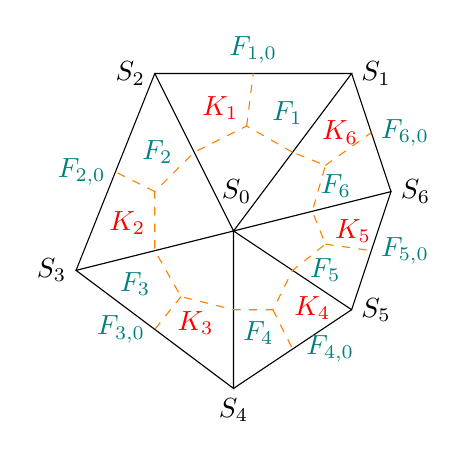
\begin{tikzpicture}[scale=0.5]
			% triangles
			\draw[-] (0,0) -- (3,4) -- (-2,4) --cycle;
			\draw[-] (0,0) -- (-4,-1) -- (0,-4) --cycle;
			\draw[-] (0,0) -- (3,-2) -- (4,1) --cycle;
			\draw[-] (-4,-1) -- (-2,4);
			\draw[-] (0,-4) -- (3,-2);
			\draw[-] (4,1) -- (3,4);
			%quadriangle
			\draw[dashed,orange] (1.5,2)--(1/3,8/3)--(-1,2)--(-2,1)--(-2,-0.5)--(-4/3,-5/3)--(0,-2)--(1,-2)--(1.5,-1)--(7/3,-1/3)--(2,0.5)--(7/3,5/3)--(1.5,2);
			\draw[dashed,orange] (1/3,8/3)--(1/2,8/2);
			\draw[dashed,orange] (-2,1)--(-3,3/2);
			\draw[dashed,orange] (-4/3,-5/3)--(-4/2,-5/2);
			\draw[dashed,orange] (1,-2)--(3/2,-3);
			\draw[dashed,orange] (7/3,-1/3)--(7/2,-1/2);
			\draw[dashed,orange] (7/3,5/3)--(7/2,5/2);
			
			% sommets
			\coordinate [label=left:$S_0$] (S_0) at (0.7,1);
			\coordinate [label=right:$S_1$] (S1) at (3,4);
			\coordinate [label=left:$S_2$] (S2) at (-2,4);
			\coordinate [label=left:$S_3$] (S3) at (-4,-1);
			\coordinate [label=below:$S_4$] (S4) at (0,-4);
			\coordinate [label=right:$S_5$] (S5) at (3,-2);
			\coordinate [label=right:$S_6$] (S6) at (4,1);
			% faces
			\coordinate [label=above:\textcolor{teal}{$F_{1,0}$}] (F1) at (1/2,4);
			\coordinate [label=left:\textcolor{teal}{$F_{2,0}$}] (F1) at (-3,1.5);
			\coordinate [label=left:\textcolor{teal}{$F_{3,0}$}] (F1) at (-2,-2.5);
			\coordinate [label=right:\textcolor{teal}{$F_{4,0}$}] (F1) at (1.6,-3);
			\coordinate [label=right:\textcolor{teal}{$F_{5,0}$}] (F1) at (3.5,-0.5);
			\coordinate [label=right:\textcolor{teal}{$F_{6,0}$}] (F1) at (3.5,2.5);
			\coordinate [label=left:\textcolor{teal}{$F_1$}] (F1) at (2,3);
			\coordinate [label = left:\textcolor{teal}{$F_2$}] (F2) at (-1.3,2);
			\coordinate [label=below:\textcolor{teal}{$F_3$}] (F3) at (-2.5,-0.8);
			\coordinate [label=right:\textcolor{teal}{$F_4$}] (F4) at (0,-2.6);
			\coordinate [label=right:\textcolor{teal}{$F_5$}] (F5) at (1.7,-1);
			\coordinate [label=above:\textcolor{teal}{$F_6$}] (F6) at (2.6,0.6);
			% Triangles
			\coordinate [label=below:\textcolor{red}{$K_1$}] (T1) at (-1/3,11/3);
			\coordinate [label=right:\textcolor{red}{$K_2$}] (T2) at (-3.4,0.2);
			\coordinate [label=right:\textcolor{red}{$K_3$}] (T3) at (-5/3,-7/3);
			\coordinate [label=above:\textcolor{red}{$K_4$}] (T4) at (2,-2.5);
			\coordinate [label=right:\textcolor{red}{$K_5$}] (T5) at (7/3,-0);
			\coordinate [label=right:\textcolor{red}{$K_6$}] (T6) at (6/3,2.5);
			\end{tikzpicture}
			\caption{Macro-element $\Mcal_0=S_1\,S_2\,S_3\,S_4\,S_5\,S_6$.}
		\end{subfigure}
		\hspace{0.2\linewidth}
		\begin{subfigure}[b]{0.39\linewidth}
			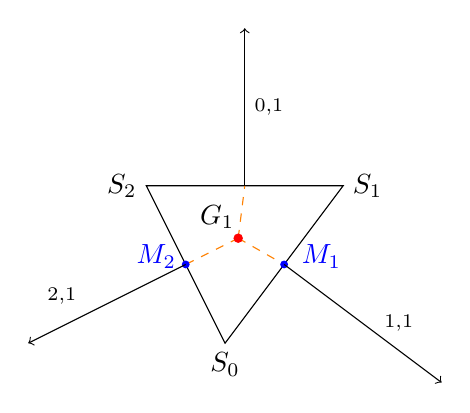
\begin{tikzpicture}[scale=0.5]
			=% triangle
			\draw[-] (0,0) -- (3,4) -- (-2,4) --cycle;
			% sommets
			\coordinate [label=below:$S_0$] (S) at (0,0);
			\coordinate [label=right:$S_1$] (S1) at (3,4);
			\coordinate [label=left:$S_2$] (S2) at (-2,4);
			% quadrangle 
			\draw[dashed,orange] (1/3,8/3)--(1.5,2);
			\draw[dashed,orange] (1/3,8/3)--(-1,2.0);
			\draw[dashed,orange] (1/3,8/3)--(1/2,4);
			% milieux des faces
			\fill[fill=blue] (-1,2) circle (0.1cm);
			\coordinate [label=left:\textcolor{blue}{$M_2$}] (M2) at (-1,2.2);
			\fill[fill=blue] (1.5,2) circle (0.1cm);
			\coordinate [label=right:\textcolor{blue}{$M_1$}] (M1) at (1.7,2.2);
			% barycentre
			\coordinate [label = above:$G_1$] (G) at (-1/5,8/3);
			\fill[fill=red] (1/3,8/3) circle (0.12cm);
			\draw [->] (1.5,2) --(5.5,-1);
			\coordinate [label = right:$\Scal_{1,1}$] (N1) at (3.8,0.5);
			\draw [->] (-1,2) -- (-5,0);
			\coordinate [label = left:$\Scal_{2,1}$] (N2) at (-3.5,1.2);
			\draw [->] (0.5,4) -- (0.5,8);
			\coordinate [label = right:$\Scal_{0,1}$] (N0) at (0.5,6);
			\end{tikzpicture}
			\caption{Triangle $K_1=S_0\,S_1\,S_2$.}
		\end{subfigure}
		\caption{Notations in case $N_{S,0}=6$ and $j\in \Ical_S^i$.}
		\label{fig:MS_and_T1}
	\end{figure}
\end{center}
\vspace{-1.1cm}
%----------------------------------------------------------%
%\subsection{Pressure gradient scheme around an inner vertex}
%----------------------------------------------------------% 
\begin{center}
	\begin{figure}[ht!]
		\begin{subfigure}[b]{0.39\linewidth}
			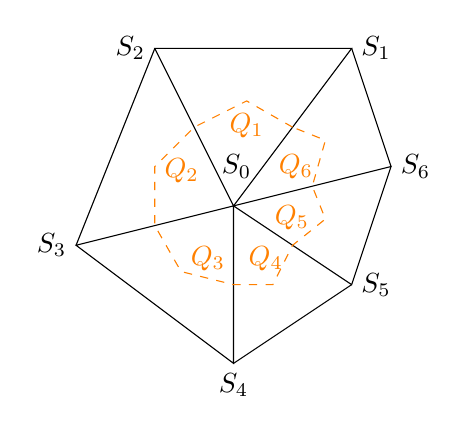
\begin{tikzpicture}[scale=0.5]
			% triangles
			\draw[-] (0,0) -- (3,4) -- (-2,4) --cycle;
			\draw[-] (0,0) -- (-4,-1) -- (0,-4) --cycle;
			\draw[-] (0,0) -- (3,-2) -- (4,1) --cycle;
			\draw[-] (-4,-1) -- (-2,4);
			\draw[-] (0,-4) -- (3,-2);
			\draw[-] (4,1) -- (3,4);
			% quadrangles
			\draw[dashed,orange] (1.5,2)--(1/3,8/3)--(-1,2)--(-2,1)--(-2,-0.5)--(-4/3,-5/3)--(0,-2)--(1,-2)--(1.5,-1)--(7/3,-1/3)--(2,0.5)--(7/3,5/3)--(1.5,2);
			% sommets
			\coordinate [label=left:$S_0$] (S) at (0.7,1);
			\coordinate [label=right:$S_1$] (S1) at (3,4);
			\coordinate [label=left:$S_2$] (S2) at (-2,4);
			\coordinate [label=left:$S_3$] (S3) at (-4,-1);
			\coordinate [label=below:$S_4$] (S4) at (0,-4);
			\coordinate [label=right:$S_5$] (S5) at (3,-2);
			\coordinate [label=right:$S_6$] (S6) at (4,1);
			%
			% quadrangles
			\coordinate [label=below:\textcolor{orange}{$Q_1$}] (Q1) at (1/3,7.8/3);
			\coordinate [label=right:\textcolor{orange}{$Q_2$}] (Q2) at (-2,0.9);
			\coordinate [label=right:\textcolor{orange}{$Q_3$}] (Q3) at (-4/3,-4/3);
			\coordinate [label=above:\textcolor{orange}{$Q_4$}] (Q4) at (0.82,-1.9);
			\coordinate [label=right:\textcolor{orange}{$Q_5$}] (Q5) at (0.80,-0.30);
			\coordinate [label=right:\textcolor{orange}{$Q_6$}] (Q6) at (0.90,1);
			\end{tikzpicture}
			\caption{Quadrangles $(Q_i)_{i=1}^{N_{S,0}}$.}
		\end{subfigure}
		\hspace{0.2\linewidth}
		\begin{subfigure}[b]{0.39\linewidth} 
			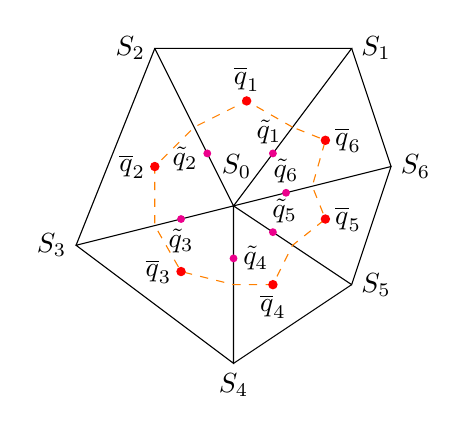
\begin{tikzpicture}[scale=0.5]
			% triangles
			\draw[-] (0,0) -- (3,4) -- (-2,4) --cycle;
			\draw[-] (0,0) -- (-4,-1) -- (0,-4) --cycle;
			\draw[-] (0,0) -- (3,-2) -- (4,1) --cycle;
			\draw[-] (-4,-1) -- (-2,4);
			\draw[-] (0,-4) -- (3,-2);
			\draw[-] (4,1) -- (3,4);
			% quadrangles
			\draw[dashed,orange] (1.5,2)--(1/3,8/3)--(-1,2)--(-2,1)--(-2,-0.5)--(-4/3,-5/3)--(0,-2)--(1,-2)--(1.5,-1)--(7/3,-1/3)--(2,0.5)--(7/3,5/3)--(1.5,2);
			% sommets
			\coordinate [label=left:$S_0$] (S) at (0.7,1);
			\coordinate [label=right:$S_1$] (S1) at (3,4);
			\coordinate [label=left:$S_2$] (S2) at (-2,4);
			\coordinate [label=left:$S_3$] (S3) at (-4,-1);
			\coordinate [label=below:$S_4$] (S4) at (0,-4);
			\coordinate [label=right:$S_5$] (S5) at (3,-2);
			\coordinate [label=right:$S_6$] (S6) at (4,1);
			%
			% Barycentres
			\coordinate [label = above:$\overline{q}_1$] (pT1) at (1/3,8/3);
			\fill[fill=red] (1/3,8/3) circle (0.12cm);
			\coordinate [label = left:$\overline{q}_2$] (pT2) at (-2,1);
			\fill[fill=red] (-2,1) circle (0.12cm);
			\coordinate [label = left:$\overline{q}_3$] (pT3) at (-4/3,-5/3);
			\fill[fill=red] (-4/3,-5/3) circle (0.12cm);
			\coordinate [label = below:$\overline{q}_4$] (pT4) at (1,-2) ;
			\fill[fill=red] (1,-2) circle (0.12cm);
			\coordinate [label = right:$\overline{q}_5$] (pT5) at (7/3,-1/3) ;
			\fill[fill=red] (7/3,-1/3) circle (0.12cm);
			\coordinate [label = right:$\overline{q}_6$] (pT6) at (7/3,5/3) ;
			\fill[fill=red] (7/3,5/3) circle (0.12cm);
			% pressions auxiliaires
			\coordinate [label = above:$\tilde{q}_1$] (p1) at (0.9,4/3);
			\fill[fill=magenta] (1,4/3) circle (0.1cm);
			\coordinate [label = left:$\tilde{q}_2$] (p2) at (-2/3,1.2);
			\fill[fill=magenta] (-2/3,4/3) circle (0.1cm);
			\coordinate [label = below:$\tilde{q}_3$] (p3) at (-4/3,-1/3);
			\fill[fill=magenta] (-4/3,-1/3) circle (0.1cm);
			\coordinate [label = right:$\tilde{q}_4$] (p4) at (0,-4/3);
			\fill[fill=magenta] (0,-4/3) circle (0.1cm);
			\coordinate [label = above:$\tilde{q}_5$] (p5) at (1.3,-0.68);
			\fill[fill=magenta] (1,-2/3) circle (0.1cm);
			\coordinate [label = above:$\tilde{q}_6$] (p6) at (4/3,1/3);
			\fill[fill=magenta] (4/3,1/3) circle (0.1cm);
			
			\end{tikzpicture}
			\caption{Discrete pressures ($\overline{q}_i$,$\tilde{q}_i)_{i=1}^{N_{S,0}}$.}
		\end{subfigure}
		\caption{MPFA Scheme for $j \in \Ical_S^i$ and $N_{S,0}=6$.}
		\label{fig:Qi}
	\end{figure}
\end{center}
\begin{center}
	\begin{figure}[h]
		\begin{subfigure}[b]{0.39\linewidth}
			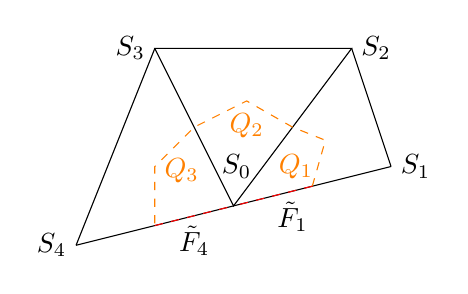
\begin{tikzpicture}[scale=0.5]
			% triangles
			\draw[-] (0,0) -- (3,4) -- (-2,4) --cycle;
			%			\draw[-] (0,0) -- (-4,-1) -- (0,-4) --cycle;
			%			\draw[-] (0,0) -- (3,-2) -- (4,1) --cycle;
			\draw[-] (-4,-1) -- (-2,4);
			%			\draw[-] (0,-4) -- (3,-2);
			\draw[-] (-4,-1) -- (4,1);
			\draw[-] (4,1) -- (3,4);
			% quadrangles
			\draw[dashed,orange] (1.5,2)--(1/3,8/3)--(-1,2)--(-2,1)--(-2,-0.5);
			\draw[dashed,orange] (2,0.5)--(7/3,5/3)--(1.5,2);
			% sommets
			\coordinate [label=left:$S_0$] (S) at (0.7,1);
			\coordinate [label=right:$S_2$] (S2) at (3,4);
			\coordinate [label=left:$S_3$] (S3) at (-2,4);
			\coordinate [label=left:$S_4$] (S4) at (-4,-1);
			%			\coordinate [label=below:$S_4$] (S4) at (0,-4);
			%			\coordinate [label=right:$S_5$] (S5) at (3,-2);
			\coordinate [label=right:$S_1$] (S1) at (4,1);
			%
			% quadrangles
			\coordinate [label=below:\textcolor{orange}{$Q_2$}] (Q2) at (1/3,7.8/3);
			\coordinate [label=right:\textcolor{orange}{$Q_3$}] (Q3) at (-2,0.9);
			%			\coordinate [label=right:\textcolor{orange}{$Q_3$}] (Q3) at (-4/3,-4/3);
			%			\coordinate [label=above:\textcolor{orange}{$Q_4$}] (Q4) at (0.82,-1.9);
			%			\coordinate [label=right:\textcolor{orange}{$Q_5$}] (Q5) at (0.80,-0.30);
			\coordinate [label=right:\textcolor{orange}{$Q_1$}] (Q1) at (0.90,1);
			% Demi-arêtes 
			\coordinate [label=below:$\tilde{F}_4$] (FI4) at (-1,-0.25);
			\coordinate [label=below:$\tilde{F}_1$] (FI1) at (6/4,0.35);
			\draw[dashed,red] (-2,-0.5)--(0,0);
			\draw[dashed,red] (2,0.5)--(0,0);
			\end{tikzpicture}
			\caption{Quadrangles $(Q_i)_{i=1}^{N_{S,0}}$.}
		\end{subfigure}
		\hspace{0.2\linewidth}
		\begin{subfigure}[b]{0.39\linewidth} 
			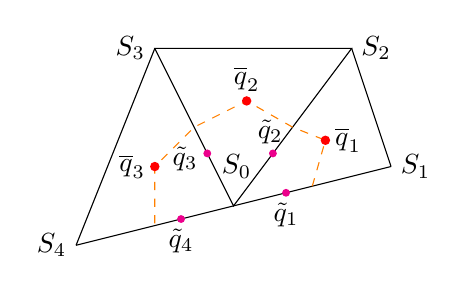
\begin{tikzpicture}[scale=0.5]
			% triangles
			\draw[-] (0,0) -- (3,4) -- (-2,4) --cycle;
			%			\draw[-] (0,0) -- (-4,-1) -- (0,-4) --cycle;
			%			\draw[-] (0,0) -- (3,-2) -- (4,1) --cycle;
			\draw[-] (-4,-1) -- (-2,4);
			%			\draw[-] (0,-4) -- (3,-2);
			\draw[-] (-4,-1) -- (4,1);
			\draw[-] (4,1) -- (3,4);
			% quadrangles
			\draw[dashed,orange] (1.5,2)--(1/3,8/3)--(-1,2)--(-2,1)--(-2,-0.5);
			\draw[dashed,orange] (2,0.5)--(7/3,5/3)--(1.5,2);
			% sommets
			\coordinate [label=left:$S_0$] (S) at (0.7,1);
			\coordinate [label=right:$S_2$] (S2) at (3,4);
			\coordinate [label=left:$S_3$] (S3) at (-2,4);
			\coordinate [label=left:$S_4$] (S4) at (-4,-1);
			%			\coordinate [label=below:$S_4$] (S4) at (0,-4);
			%			\coordinate [label=right:$S_5$] (S5) at (3,-2);
			\coordinate [label=right:$S_1$] (S1) at (4,1);
			%
			% Barycentres
			\coordinate [label = above:$\overline{q}_2$] (pT2) at (1/3,8/3);
			\fill[fill=red] (1/3,8/3) circle (0.12cm);
			\coordinate [label = left:$\overline{q}_3$] (pT3) at (-2,1);
			\fill[fill=red] (-2,1) circle (0.12cm);
			%			\coordinate [label = left:$\overline{p}_3$] (pT3) at (-4/3,-5/3);
			%			\fill[fill=red] (-4/3,-5/3) circle (0.12cm);
			%			\coordinate [label = below:$\overline{p}_4$] (pT4) at (1,-2) ;
			%			\fill[fill=red] (1,-2) circle (0.12cm);
			%			\coordinate [label = right:$\overline{p}_5$] (pT5) at (7/3,-1/3) ;
			%			\fill[fill=red] (7/3,-1/3) circle (0.12cm);
			\coordinate [label = right:$\overline{q}_1$] (pT1) at (7/3,5/3) ;
			\fill[fill=red] (7/3,5/3) circle (0.12cm);
			% pressions auxiliaires
			\coordinate [label = above:$\tilde{q}_2$] (p2) at (0.93,4/3);
			\fill[fill=magenta] (1,4/3) circle (0.1cm);
			\coordinate [label = left:$\tilde{q}_3$] (p3) at (-2/3,1.2);
			\fill[fill=magenta] (-2/3,4/3) circle (0.1cm);
			\coordinate [label = below:$\tilde{q}_4$] (p4) at (-4/3,-1/3);
			\fill[fill=magenta] (-4/3,-1/3) circle (0.1cm);
			%			\coordinate [label = right:$\tilde{p}_4$] (p4) at (0,-4/3);
			%			\fill[fill=magenta] (0,-4/3) circle (0.1cm);
			%			\coordinate [label = above:$\tilde{p}_5$] (p5) at (1,-2/3);
			%			\fill[fill=magenta] (1,-2/3) circle (0.1cm);
			\coordinate [label = below:$\tilde{q}_1$] (p1) at (4/3,1/3);
			\fill[fill=magenta] (4/3,1/3) circle (0.1cm);
			
			\end{tikzpicture}
			\caption{Discrete pressures ($\overline{q}_i$,$\tilde{q}_i)_{i=1}^{N_{S,0}}$.}
		\end{subfigure}
		\caption{MPFA Scheme for $j \in \Ical_S^b$ and $N_{S,0}=4$ }
		\label{fig:Qj}
	\end{figure}
\end{center}
\vspace{-0.5cm}
Let $q_h\in Q_h$. We set $q_{h|K_\ell}:=\ov{q}_\ell$.
\\
Consider $S_0\in\Om$ (Fig. \ref{fig:Qi}). Let us build a piecewise affine approximation of $q_h$ on each quadrangle $(Q_i)_{i=1}^{N_{S,0}}$ (see Fig. \ref{fig:Qi}-(a)). We call this approximation $\tilde{q}_h$. We first introduce auxiliary discrete pressure values $(\tilde{q}_i)_{i=1}^{N_{S,0}}$ on the thirds of the inner edges of $\Mcal_0$ (see Fig. \ref{fig:Qi}-(b)). For all $j\in\Ical_{S,i}$, we define $\Gcal_i(q_h):=\grad\tilde{q}_{h|Q_i}$, using an integration by part as it is done in \cite[Sect. 3]{LEPOTIER05bis} and \cite[Sect. 1.1.1]{lepotierhdr}: % $\ds\frac{\Scal_{i,i+1}}{d}$: 
$$ |Q_i| \Gcal_i= \int_{Q_i} \Gcal_i(q_h) = \int_{\partial Q_i} \tilde{q}_h  \nvec_{\partial Q_i}=\, \tilde{q}_i \frac{\Scal_{i,i}}{d} + \tilde{q}_{i+1}\,\frac{\Scal_{i+1,i}}{d}  + \ov{q}_i(-\frac{\Scal_{i,i}}{d}-\frac{\Scal_{i+1,i}}{d}). $$ 


Hence, noticing that $|Q_i|= \frac{|T_i|}{d+1}$, we have:
\begin{equation}\label{eq:gradientlocal1}
\Gcal_i(q_h)=\ds\frac{1}{|Q_i|}\left(\,(\tilde{q}_i-\ov{q}_i)\,\frac{\Scal_{i,i}}{d}+(\tilde{q}_{i+1}-\ov{q}_i)\,\frac{\Scal_{i+1,i}}{d}\right) =\ds\frac{d+1}{d\,|T_i|}\left(\,\tilde{q}_i\,\Scal_{i,i}+\tilde{q}_{i+1}\,\Scal_{i+1,i}+\ov{q}_i\,\Scal_{0,i}\,\right).
\end{equation}
In order to preserve the flux across the inner edges of $\Mcal_0$, we write that:
%--------------%
\begin{equation}\label{eq:continuitefacesnormales}
\forall i\in\Ical_{S,0},\quad \Gcal_i(q_h)\cdot\Scal_{i+1,i}+\Gcal_{i+1}(q_h)\cdot\Scal_{i+1,i+1}=0.
\end{equation}
These $N_{S,0}$ equations with $N_{S,0}$ unknowns (the auxiliary discrete pressure values $(\tilde{q}_i)_{i=1}^{N_{S,0}}$) lead to a well posed linear system. Thus, we can evaluate the auxiliary discrete pressure values $(\tilde{q}_i)_{i=1}^{N_{S,0}}$ with the data $(\ov{q}_i)_{i=1}^{N_{S,0}}$. Therefore, we can explicitly express the pressure gradients $(\Gcal_i(q_h))_{i=1}^{N_{S,0}}$ \eqref{eq:gradientlocal1}.
\\
Consider now $S_0\in\pa\Om$ (see Fig. \ref{fig:Qj}).  According to \cite[proof of Prop. IV.3.7]{BoyerFabrie12}, if $\fvec\in\bH^1(\Om)$, the solution $(\uvec,p)$ to Problem \eqref{eq:Stokes} is such that:
\begin{equation}\label{eq:Stokes-FVh-P0}
\grad p \cdot \nvec_{|\partial \Omega}=\fvec\cdot \nvec_{|\partial \Omega},
\end{equation}
where $\nvec_{|\partial \Omega}$ is the unit outward normal vector at $\partial \Omega$. 

In our numerical experiments, we explicit the auxiliary discrete pressure values located on $\pa\Om$ (ie $\tilde{q}_1$ and $\tilde{q}_4$ on Fig. \ref{fig:Qj}-(b)) by imposing that for all $i\in\Ical_{S,0}$ such that $F_i\in\pa\Om$:
\begin{equation}
\label{eq:grap.n=f.n}
\int_{\tilde{F}_i}  \Gcal_i(q_h)\cdot\nvec_{|\tilde{F}_i}= \int_{\tilde{F}_i} \fvec\cdot \nvec_{|\tilde{F}_i}.
\end{equation}
Again, the auxiliary discrete pressure values solve a well posed linear system. They can be written with the data $(\ov{q}_i)_{i=1}^{N_{S,0}}$ and we can explicitly express $\Gcal_i(q_h)$.
\\

For $i\in\Ical_S$, we let $(Q_{i,j})_j\in\Ical_{S,i}$ be the set of quadrangles built around $S_i$, and we call $\mathcal{Q}_h$ the mesh of all the quadrangles $\mathcal{Q}_h:=(\,(Q_{i,j})_{j\in\Ical_{S,i}})_{i\in\Ical_S}$. Let $q_h\in Q_h$. Let $i\in\Ical_S$. In the macro-element $\Mcal_i$, we call $\Gcal_{i,j}(q_h)$ the local reconstructed gradient of $q_h$. We now define the MPFA gradient reconstruction as the operator $\Gcal_h$: 

\begin{equation}
\label{eq:gradientMPFA}
\Gcal_h:\left\{
\begin{array}{rcl}Q_h&\rightarrow&\bP^0(\mathcal{Q}_h)\\
q_h&\mapsto&\Gcal_h(q_h)
\end{array}\right.
\,|\quad  \forall  i\in\Ical_S, \,  \forall j \in \Ical_{S,i},\quad
\Gcal_h(q_h)_{|Q_{i,j}} = \Gcal_{i,j}(q_{h|\Mcal_i}).
\end{equation}
If the data $\fvec$ is of low regularity, one can enhance the space of discrete pressures, adding the auxiliary unknowns on the boundary as degrees of freedom.
\\


\begin{prop}
	With triangles, and $p\in C^2(\Om)$, the fluxes of the symmetric MPFA scheme are consistently approximated. Also by choosing the auxiliary pressures unknowns at the thirds of the edges, the gradient is approximated exactly for affine functions. Also, the symmetric MPFA scheme is  consistent, coercive and convergent. 
\end{prop} 
The proof of this proposition can be found in \cite[Prop. 2, Prop. 3 ]{LEPOTIER05bis} and \cite[Theorem 3.2]{LiShYo09}.\\



Let us express our discrete Stokes problem. Let $g_h(\cdot,\cdot)$ be the following bilinear form:
\begin{equation}\label{eq:bilin-form-gh}
g_h:\left\{
\begin{array}{rcl}
\bX_{h}\times Q_h&\rightarrow&\R\\
(\vvec_h,q_h)&\mapsto&(\Gcal_h(q_h),\vvec_h)_{\bL^2(\Om)}
\end{array}
\right..
\end{equation}

The discretization of \eqref{eq:Stokes} using the MPFA scheme to discretize the pressure gradient reads:
\begin{equation}
\label{eq:MPFA-VF}
\mbox{Find }(\uvec,p)\in\bX_{0,h}\times Q_h\,|\quad \left\{
\begin{array}{rcll}
a_{\nu,h}(\uvec_h, \vvec_h)+g_h(\vvec_h, p_h)&=&(\fvec, \vvec_h)_{\bL^2(\Om)} & \forall \vvec_h \in  \textbf{X}_h\\
b_h(\uvec_h, q_h)&=&0 &\forall q_h \in Q_h
\end{array}
\right.,
\end{equation}
where the bilinear forms $a_{\nu,h}(\cdot,\cdot)$ and $b_h(\cdot,\cdot)$ are defined by \eqref{eq:DiscBilinForms}. Notice that the linear system related to variational formulation \eqref{eq:MPFA-VF} is not symmetric.






 
%%---------------------------------------------------------%
\section{The $\bP^1_{nc}-P^0_{Mps}$ scheme}\label{sec:MPFA}

Here, we use the symmetric MPFA scheme (where MPFA stands for {\em multi-points flux approximation}) to discretize the pressure gradient term in \eqref{eq:Stokes}, in the case of a simplicial mesh. The discrete pressure space remains $Q_h=Q_{0,h}$. We call this new scheme the $\bP^1_{nc}-P^0_{Mps}$ scheme.
\par
Let us consider the $2D$ case.
To design the scheme, as it has been initially done in \cite{LEPOTIER05bis, LEPOTIER05}, we start by splitting the triangles into three quadrangles, connecting the barycentre of the triangle to the midpoint of each edges. Considering some $ q_h \in Q_h$, we will calculate an affine approximation of $Q_h$ on each quadrangles. To do so,we need to add temporary auxiliary unknowns located on the third of the edges.
\\
%-----------------------------------------%
%\subsection{Notations and dual mesh in $2D$}
%-----------------------------------------%
Let us introduce some notations. \\

Let  $j \in \Ical_{S}$. We define the macro-element $\Mcal_j$ such that $\ds\overline{\Mcal}_j:=\bigcap_{\ell\in\Ical_{K,j}}\overline{K}_\ell$. Let renumber the vertices so that: $S_0=S_j$, $\Ical_{S,0}=\{1,\cdots,N_{S,0}\}$ and for all $i\in\Ical_{S,0}$, $S_iS_{i+1}\in\Fcal_h$ (setting $S_{N_{S,0}+1}=S_{N_{S,0}}$). For $i\in\Ical_{S,0}$ we denote by:
\begin{itemize}
	\item $K_i$ the triangle of vertices $S_0 S_i S_{i+1}$, and we call its barycentre $G_i$.
	\item $F_i$ the edge such that $F_i=S_0S_i$, and we call $M_i$ its midpoint. 
	\item $F_{i,0}$ the edge opposite to $S_0$ in $K_i$. 
	\item $\tilde{F}_i$ the half-edges defined by $S_0$ and the midpoint of $F_i$.
	\item $Q_i$ the quadrangle of vertices $S_0\,M_i\,G_i\,M_{i+1}$ (Fig. \ref{fig:Qi}-(a) for $S_0\in\Om$ and \ref{fig:Qj}-(a) for $S_0\in\pa\Om$).
\end{itemize}
For $i,\,j\in\Ical_{S,0}$, we denote by $\Scal_{i,j}$ the normal vector outgoing of $K_j$ at $F_i$ and of norm $|F_i|$. For $i\in\Ical_{S,0}$, we call $\Scal_{0,i}$ the normal vector outgoing of $K_i$ at $F_{i,0}$. On Figure \ref{fig:MS_and_T1}-(a), we represent $\Mcal_0$ in case $S_0\in\Om$ and $N_{S,0}=6$. On Figure \ref{fig:MS_and_T1}-(b), we represent the triangle $K_1$ with the vectors $(\Scal_{j,1})_{j=0}^2$ and its barycentre $G_1$.
\vspace{-0.3cm}
\begin{center}
	\begin{figure}[ht!]
		\begin{subfigure}[b]{0.39\linewidth}
			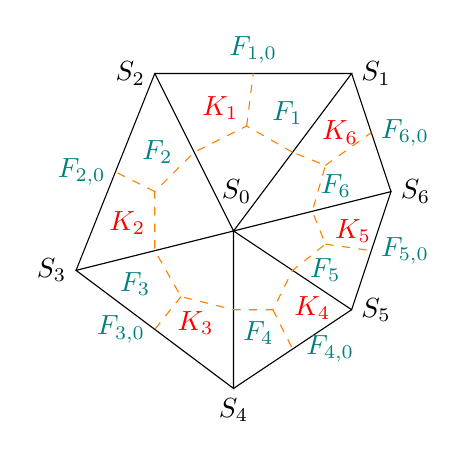
\begin{tikzpicture}[scale=0.5]
			% triangles
			\draw[-] (0,0) -- (3,4) -- (-2,4) --cycle;
			\draw[-] (0,0) -- (-4,-1) -- (0,-4) --cycle;
			\draw[-] (0,0) -- (3,-2) -- (4,1) --cycle;
			\draw[-] (-4,-1) -- (-2,4);
			\draw[-] (0,-4) -- (3,-2);
			\draw[-] (4,1) -- (3,4);
			%quadriangle
			\draw[dashed,orange] (1.5,2)--(1/3,8/3)--(-1,2)--(-2,1)--(-2,-0.5)--(-4/3,-5/3)--(0,-2)--(1,-2)--(1.5,-1)--(7/3,-1/3)--(2,0.5)--(7/3,5/3)--(1.5,2);
			\draw[dashed,orange] (1/3,8/3)--(1/2,8/2);
			\draw[dashed,orange] (-2,1)--(-3,3/2);
			\draw[dashed,orange] (-4/3,-5/3)--(-4/2,-5/2);
			\draw[dashed,orange] (1,-2)--(3/2,-3);
			\draw[dashed,orange] (7/3,-1/3)--(7/2,-1/2);
			\draw[dashed,orange] (7/3,5/3)--(7/2,5/2);
			
			% sommets
			\coordinate [label=left:$S_0$] (S_0) at (0.7,1);
			\coordinate [label=right:$S_1$] (S1) at (3,4);
			\coordinate [label=left:$S_2$] (S2) at (-2,4);
			\coordinate [label=left:$S_3$] (S3) at (-4,-1);
			\coordinate [label=below:$S_4$] (S4) at (0,-4);
			\coordinate [label=right:$S_5$] (S5) at (3,-2);
			\coordinate [label=right:$S_6$] (S6) at (4,1);
			% faces
			\coordinate [label=above:\textcolor{teal}{$F_{1,0}$}] (F1) at (1/2,4);
			\coordinate [label=left:\textcolor{teal}{$F_{2,0}$}] (F1) at (-3,1.5);
			\coordinate [label=left:\textcolor{teal}{$F_{3,0}$}] (F1) at (-2,-2.5);
			\coordinate [label=right:\textcolor{teal}{$F_{4,0}$}] (F1) at (1.6,-3);
			\coordinate [label=right:\textcolor{teal}{$F_{5,0}$}] (F1) at (3.5,-0.5);
			\coordinate [label=right:\textcolor{teal}{$F_{6,0}$}] (F1) at (3.5,2.5);
			\coordinate [label=left:\textcolor{teal}{$F_1$}] (F1) at (2,3);
			\coordinate [label = left:\textcolor{teal}{$F_2$}] (F2) at (-1.3,2);
			\coordinate [label=below:\textcolor{teal}{$F_3$}] (F3) at (-2.5,-0.8);
			\coordinate [label=right:\textcolor{teal}{$F_4$}] (F4) at (0,-2.6);
			\coordinate [label=right:\textcolor{teal}{$F_5$}] (F5) at (1.7,-1);
			\coordinate [label=above:\textcolor{teal}{$F_6$}] (F6) at (2.6,0.6);
			% Triangles
			\coordinate [label=below:\textcolor{red}{$K_1$}] (T1) at (-1/3,11/3);
			\coordinate [label=right:\textcolor{red}{$K_2$}] (T2) at (-3.4,0.2);
			\coordinate [label=right:\textcolor{red}{$K_3$}] (T3) at (-5/3,-7/3);
			\coordinate [label=above:\textcolor{red}{$K_4$}] (T4) at (2,-2.5);
			\coordinate [label=right:\textcolor{red}{$K_5$}] (T5) at (7/3,-0);
			\coordinate [label=right:\textcolor{red}{$K_6$}] (T6) at (6/3,2.5);
			\end{tikzpicture}
			\caption{Macro-element $\Mcal_0=S_1\,S_2\,S_3\,S_4\,S_5\,S_6$.}
		\end{subfigure}
		\hspace{0.2\linewidth}
		\begin{subfigure}[b]{0.39\linewidth}
			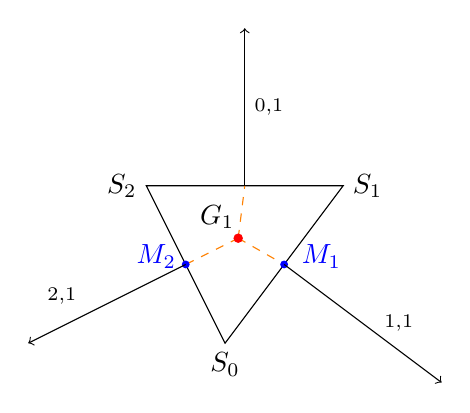
\begin{tikzpicture}[scale=0.5]
			=% triangle
			\draw[-] (0,0) -- (3,4) -- (-2,4) --cycle;
			% sommets
			\coordinate [label=below:$S_0$] (S) at (0,0);
			\coordinate [label=right:$S_1$] (S1) at (3,4);
			\coordinate [label=left:$S_2$] (S2) at (-2,4);
			% quadrangle 
			\draw[dashed,orange] (1/3,8/3)--(1.5,2);
			\draw[dashed,orange] (1/3,8/3)--(-1,2.0);
			\draw[dashed,orange] (1/3,8/3)--(1/2,4);
			% milieux des faces
			\fill[fill=blue] (-1,2) circle (0.1cm);
			\coordinate [label=left:\textcolor{blue}{$M_2$}] (M2) at (-1,2.2);
			\fill[fill=blue] (1.5,2) circle (0.1cm);
			\coordinate [label=right:\textcolor{blue}{$M_1$}] (M1) at (1.7,2.2);
			% barycentre
			\coordinate [label = above:$G_1$] (G) at (-1/5,8/3);
			\fill[fill=red] (1/3,8/3) circle (0.12cm);
			\draw [->] (1.5,2) --(5.5,-1);
			\coordinate [label = right:$\Scal_{1,1}$] (N1) at (3.8,0.5);
			\draw [->] (-1,2) -- (-5,0);
			\coordinate [label = left:$\Scal_{2,1}$] (N2) at (-3.5,1.2);
			\draw [->] (0.5,4) -- (0.5,8);
			\coordinate [label = right:$\Scal_{0,1}$] (N0) at (0.5,6);
			\end{tikzpicture}
			\caption{Triangle $K_1=S_0\,S_1\,S_2$.}
		\end{subfigure}
		\caption{Notations in case $N_{S,0}=6$ and $j\in \Ical_S^i$.}
		\label{fig:MS_and_T1}
	\end{figure}
\end{center}
\vspace{-1.1cm}
%----------------------------------------------------------%
%\subsection{Pressure gradient scheme around an inner vertex}
%----------------------------------------------------------% 
\begin{center}
	\begin{figure}[ht!]
		\begin{subfigure}[b]{0.39\linewidth}
			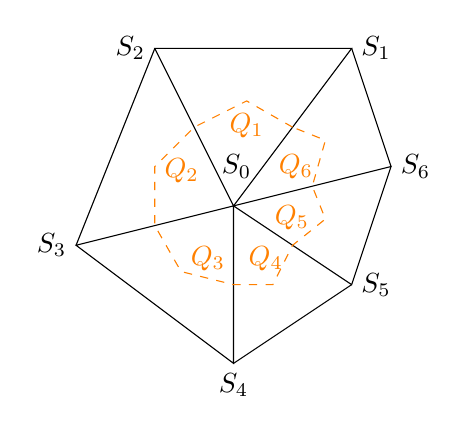
\begin{tikzpicture}[scale=0.5]
			% triangles
			\draw[-] (0,0) -- (3,4) -- (-2,4) --cycle;
			\draw[-] (0,0) -- (-4,-1) -- (0,-4) --cycle;
			\draw[-] (0,0) -- (3,-2) -- (4,1) --cycle;
			\draw[-] (-4,-1) -- (-2,4);
			\draw[-] (0,-4) -- (3,-2);
			\draw[-] (4,1) -- (3,4);
			% quadrangles
			\draw[dashed,orange] (1.5,2)--(1/3,8/3)--(-1,2)--(-2,1)--(-2,-0.5)--(-4/3,-5/3)--(0,-2)--(1,-2)--(1.5,-1)--(7/3,-1/3)--(2,0.5)--(7/3,5/3)--(1.5,2);
			% sommets
			\coordinate [label=left:$S_0$] (S) at (0.7,1);
			\coordinate [label=right:$S_1$] (S1) at (3,4);
			\coordinate [label=left:$S_2$] (S2) at (-2,4);
			\coordinate [label=left:$S_3$] (S3) at (-4,-1);
			\coordinate [label=below:$S_4$] (S4) at (0,-4);
			\coordinate [label=right:$S_5$] (S5) at (3,-2);
			\coordinate [label=right:$S_6$] (S6) at (4,1);
			%
			% quadrangles
			\coordinate [label=below:\textcolor{orange}{$Q_1$}] (Q1) at (1/3,7.8/3);
			\coordinate [label=right:\textcolor{orange}{$Q_2$}] (Q2) at (-2,0.9);
			\coordinate [label=right:\textcolor{orange}{$Q_3$}] (Q3) at (-4/3,-4/3);
			\coordinate [label=above:\textcolor{orange}{$Q_4$}] (Q4) at (0.82,-1.9);
			\coordinate [label=right:\textcolor{orange}{$Q_5$}] (Q5) at (0.80,-0.30);
			\coordinate [label=right:\textcolor{orange}{$Q_6$}] (Q6) at (0.90,1);
			\end{tikzpicture}
			\caption{Quadrangles $(Q_i)_{i=1}^{N_{S,0}}$.}
		\end{subfigure}
		\hspace{0.2\linewidth}
		\begin{subfigure}[b]{0.39\linewidth} 
			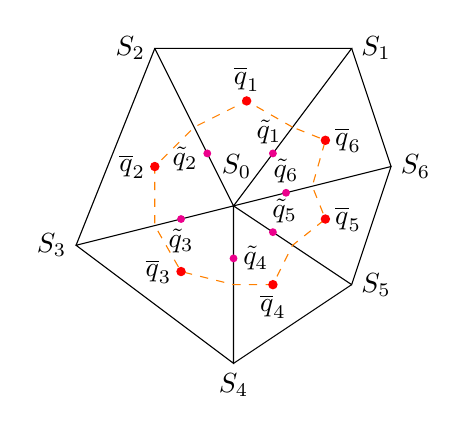
\begin{tikzpicture}[scale=0.5]
			% triangles
			\draw[-] (0,0) -- (3,4) -- (-2,4) --cycle;
			\draw[-] (0,0) -- (-4,-1) -- (0,-4) --cycle;
			\draw[-] (0,0) -- (3,-2) -- (4,1) --cycle;
			\draw[-] (-4,-1) -- (-2,4);
			\draw[-] (0,-4) -- (3,-2);
			\draw[-] (4,1) -- (3,4);
			% quadrangles
			\draw[dashed,orange] (1.5,2)--(1/3,8/3)--(-1,2)--(-2,1)--(-2,-0.5)--(-4/3,-5/3)--(0,-2)--(1,-2)--(1.5,-1)--(7/3,-1/3)--(2,0.5)--(7/3,5/3)--(1.5,2);
			% sommets
			\coordinate [label=left:$S_0$] (S) at (0.7,1);
			\coordinate [label=right:$S_1$] (S1) at (3,4);
			\coordinate [label=left:$S_2$] (S2) at (-2,4);
			\coordinate [label=left:$S_3$] (S3) at (-4,-1);
			\coordinate [label=below:$S_4$] (S4) at (0,-4);
			\coordinate [label=right:$S_5$] (S5) at (3,-2);
			\coordinate [label=right:$S_6$] (S6) at (4,1);
			%
			% Barycentres
			\coordinate [label = above:$\overline{q}_1$] (pT1) at (1/3,8/3);
			\fill[fill=red] (1/3,8/3) circle (0.12cm);
			\coordinate [label = left:$\overline{q}_2$] (pT2) at (-2,1);
			\fill[fill=red] (-2,1) circle (0.12cm);
			\coordinate [label = left:$\overline{q}_3$] (pT3) at (-4/3,-5/3);
			\fill[fill=red] (-4/3,-5/3) circle (0.12cm);
			\coordinate [label = below:$\overline{q}_4$] (pT4) at (1,-2) ;
			\fill[fill=red] (1,-2) circle (0.12cm);
			\coordinate [label = right:$\overline{q}_5$] (pT5) at (7/3,-1/3) ;
			\fill[fill=red] (7/3,-1/3) circle (0.12cm);
			\coordinate [label = right:$\overline{q}_6$] (pT6) at (7/3,5/3) ;
			\fill[fill=red] (7/3,5/3) circle (0.12cm);
			% pressions auxiliaires
			\coordinate [label = above:$\tilde{q}_1$] (p1) at (0.9,4/3);
			\fill[fill=magenta] (1,4/3) circle (0.1cm);
			\coordinate [label = left:$\tilde{q}_2$] (p2) at (-2/3,1.2);
			\fill[fill=magenta] (-2/3,4/3) circle (0.1cm);
			\coordinate [label = below:$\tilde{q}_3$] (p3) at (-4/3,-1/3);
			\fill[fill=magenta] (-4/3,-1/3) circle (0.1cm);
			\coordinate [label = right:$\tilde{q}_4$] (p4) at (0,-4/3);
			\fill[fill=magenta] (0,-4/3) circle (0.1cm);
			\coordinate [label = above:$\tilde{q}_5$] (p5) at (1.3,-0.68);
			\fill[fill=magenta] (1,-2/3) circle (0.1cm);
			\coordinate [label = above:$\tilde{q}_6$] (p6) at (4/3,1/3);
			\fill[fill=magenta] (4/3,1/3) circle (0.1cm);
			
			\end{tikzpicture}
			\caption{Discrete pressures ($\overline{q}_i$,$\tilde{q}_i)_{i=1}^{N_{S,0}}$.}
		\end{subfigure}
		\caption{MPFA Scheme for $j \in \Ical_S^i$ and $N_{S,0}=6$.}
		\label{fig:Qi}
	\end{figure}
\end{center}
\begin{center}
	\begin{figure}[h]
		\begin{subfigure}[b]{0.39\linewidth}
			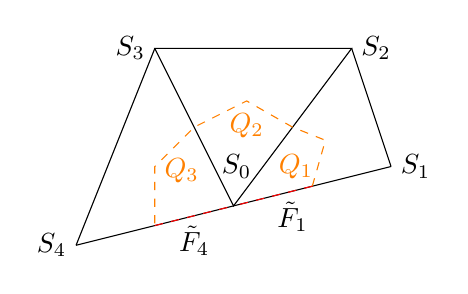
\begin{tikzpicture}[scale=0.5]
			% triangles
			\draw[-] (0,0) -- (3,4) -- (-2,4) --cycle;
			%			\draw[-] (0,0) -- (-4,-1) -- (0,-4) --cycle;
			%			\draw[-] (0,0) -- (3,-2) -- (4,1) --cycle;
			\draw[-] (-4,-1) -- (-2,4);
			%			\draw[-] (0,-4) -- (3,-2);
			\draw[-] (-4,-1) -- (4,1);
			\draw[-] (4,1) -- (3,4);
			% quadrangles
			\draw[dashed,orange] (1.5,2)--(1/3,8/3)--(-1,2)--(-2,1)--(-2,-0.5);
			\draw[dashed,orange] (2,0.5)--(7/3,5/3)--(1.5,2);
			% sommets
			\coordinate [label=left:$S_0$] (S) at (0.7,1);
			\coordinate [label=right:$S_2$] (S2) at (3,4);
			\coordinate [label=left:$S_3$] (S3) at (-2,4);
			\coordinate [label=left:$S_4$] (S4) at (-4,-1);
			%			\coordinate [label=below:$S_4$] (S4) at (0,-4);
			%			\coordinate [label=right:$S_5$] (S5) at (3,-2);
			\coordinate [label=right:$S_1$] (S1) at (4,1);
			%
			% quadrangles
			\coordinate [label=below:\textcolor{orange}{$Q_2$}] (Q2) at (1/3,7.8/3);
			\coordinate [label=right:\textcolor{orange}{$Q_3$}] (Q3) at (-2,0.9);
			%			\coordinate [label=right:\textcolor{orange}{$Q_3$}] (Q3) at (-4/3,-4/3);
			%			\coordinate [label=above:\textcolor{orange}{$Q_4$}] (Q4) at (0.82,-1.9);
			%			\coordinate [label=right:\textcolor{orange}{$Q_5$}] (Q5) at (0.80,-0.30);
			\coordinate [label=right:\textcolor{orange}{$Q_1$}] (Q1) at (0.90,1);
			% Demi-arêtes 
			\coordinate [label=below:$\tilde{F}_4$] (FI4) at (-1,-0.25);
			\coordinate [label=below:$\tilde{F}_1$] (FI1) at (6/4,0.35);
			\draw[dashed,red] (-2,-0.5)--(0,0);
			\draw[dashed,red] (2,0.5)--(0,0);
			\end{tikzpicture}
			\caption{Quadrangles $(Q_i)_{i=1}^{N_{S,0}}$.}
		\end{subfigure}
		\hspace{0.2\linewidth}
		\begin{subfigure}[b]{0.39\linewidth} 
			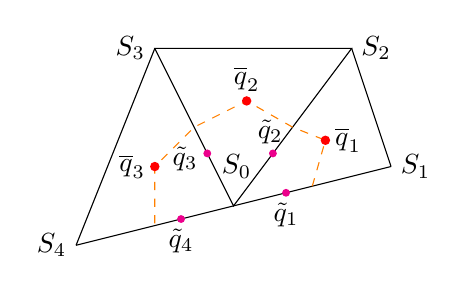
\begin{tikzpicture}[scale=0.5]
			% triangles
			\draw[-] (0,0) -- (3,4) -- (-2,4) --cycle;
			%			\draw[-] (0,0) -- (-4,-1) -- (0,-4) --cycle;
			%			\draw[-] (0,0) -- (3,-2) -- (4,1) --cycle;
			\draw[-] (-4,-1) -- (-2,4);
			%			\draw[-] (0,-4) -- (3,-2);
			\draw[-] (-4,-1) -- (4,1);
			\draw[-] (4,1) -- (3,4);
			% quadrangles
			\draw[dashed,orange] (1.5,2)--(1/3,8/3)--(-1,2)--(-2,1)--(-2,-0.5);
			\draw[dashed,orange] (2,0.5)--(7/3,5/3)--(1.5,2);
			% sommets
			\coordinate [label=left:$S_0$] (S) at (0.7,1);
			\coordinate [label=right:$S_2$] (S2) at (3,4);
			\coordinate [label=left:$S_3$] (S3) at (-2,4);
			\coordinate [label=left:$S_4$] (S4) at (-4,-1);
			%			\coordinate [label=below:$S_4$] (S4) at (0,-4);
			%			\coordinate [label=right:$S_5$] (S5) at (3,-2);
			\coordinate [label=right:$S_1$] (S1) at (4,1);
			%
			% Barycentres
			\coordinate [label = above:$\overline{q}_2$] (pT2) at (1/3,8/3);
			\fill[fill=red] (1/3,8/3) circle (0.12cm);
			\coordinate [label = left:$\overline{q}_3$] (pT3) at (-2,1);
			\fill[fill=red] (-2,1) circle (0.12cm);
			%			\coordinate [label = left:$\overline{p}_3$] (pT3) at (-4/3,-5/3);
			%			\fill[fill=red] (-4/3,-5/3) circle (0.12cm);
			%			\coordinate [label = below:$\overline{p}_4$] (pT4) at (1,-2) ;
			%			\fill[fill=red] (1,-2) circle (0.12cm);
			%			\coordinate [label = right:$\overline{p}_5$] (pT5) at (7/3,-1/3) ;
			%			\fill[fill=red] (7/3,-1/3) circle (0.12cm);
			\coordinate [label = right:$\overline{q}_1$] (pT1) at (7/3,5/3) ;
			\fill[fill=red] (7/3,5/3) circle (0.12cm);
			% pressions auxiliaires
			\coordinate [label = above:$\tilde{q}_2$] (p2) at (0.93,4/3);
			\fill[fill=magenta] (1,4/3) circle (0.1cm);
			\coordinate [label = left:$\tilde{q}_3$] (p3) at (-2/3,1.2);
			\fill[fill=magenta] (-2/3,4/3) circle (0.1cm);
			\coordinate [label = below:$\tilde{q}_4$] (p4) at (-4/3,-1/3);
			\fill[fill=magenta] (-4/3,-1/3) circle (0.1cm);
			%			\coordinate [label = right:$\tilde{p}_4$] (p4) at (0,-4/3);
			%			\fill[fill=magenta] (0,-4/3) circle (0.1cm);
			%			\coordinate [label = above:$\tilde{p}_5$] (p5) at (1,-2/3);
			%			\fill[fill=magenta] (1,-2/3) circle (0.1cm);
			\coordinate [label = below:$\tilde{q}_1$] (p1) at (4/3,1/3);
			\fill[fill=magenta] (4/3,1/3) circle (0.1cm);
			
			\end{tikzpicture}
			\caption{Discrete pressures ($\overline{q}_i$,$\tilde{q}_i)_{i=1}^{N_{S,0}}$.}
		\end{subfigure}
		\caption{MPFA Scheme for $j \in \Ical_S^b$ and $N_{S,0}=4$ }
		\label{fig:Qj}
	\end{figure}
\end{center}
\vspace{-0.5cm}
Let $q_h\in Q_h$. We set $q_{h|K_\ell}:=\ov{q}_\ell$.
\\
Consider $S_0\in\Om$ (Fig. \ref{fig:Qi}). Let us build a piecewise affine approximation of $q_h$ on each quadrangle $(Q_i)_{i=1}^{N_{S,0}}$ (see Fig. \ref{fig:Qi}-(a)). We call this approximation $\tilde{q}_h$. We first introduce auxiliary discrete pressure values $(\tilde{q}_i)_{i=1}^{N_{S,0}}$ on the thirds of the inner edges of $\Mcal_0$ (see Fig. \ref{fig:Qi}-(b)). For all $j\in\Ical_{S,i}$, we define $\Gcal_i(q_h):=\grad\tilde{q}_{h|Q_i}$, using an integration by part as it is done in \cite[Sect. 3]{LEPOTIER05bis} and \cite[Sect. 1.1.1]{lepotierhdr}: % $\ds\frac{\Scal_{i,i+1}}{d}$: 
$$ |Q_i| \Gcal_i= \int_{Q_i} \Gcal_i(q_h) = \int_{\partial Q_i} \tilde{q}_h  \nvec_{\partial Q_i}=\, \tilde{q}_i \frac{\Scal_{i,i}}{d} + \tilde{q}_{i+1}\,\frac{\Scal_{i+1,i}}{d}  + \ov{q}_i(-\frac{\Scal_{i,i}}{d}-\frac{\Scal_{i+1,i}}{d}). $$ 


Hence, noticing that $|Q_i|= \frac{|T_i|}{d+1}$, we have:
\begin{equation}\label{eq:gradientlocal1}
\Gcal_i(q_h)=\ds\frac{1}{|Q_i|}\left(\,(\tilde{q}_i-\ov{q}_i)\,\frac{\Scal_{i,i}}{d}+(\tilde{q}_{i+1}-\ov{q}_i)\,\frac{\Scal_{i+1,i}}{d}\right) =\ds\frac{d+1}{d\,|T_i|}\left(\,\tilde{q}_i\,\Scal_{i,i}+\tilde{q}_{i+1}\,\Scal_{i+1,i}+\ov{q}_i\,\Scal_{0,i}\,\right).
\end{equation}
In order to preserve the flux across the inner edges of $\Mcal_0$, we write that:
%--------------%
\begin{equation}\label{eq:continuitefacesnormales}
\forall i\in\Ical_{S,0},\quad \Gcal_i(q_h)\cdot\Scal_{i+1,i}+\Gcal_{i+1}(q_h)\cdot\Scal_{i+1,i+1}=0.
\end{equation}
These $N_{S,0}$ equations with $N_{S,0}$ unknowns (the auxiliary discrete pressure values $(\tilde{q}_i)_{i=1}^{N_{S,0}}$) lead to a well posed linear system. Thus, we can evaluate the auxiliary discrete pressure values $(\tilde{q}_i)_{i=1}^{N_{S,0}}$ with the data $(\ov{q}_i)_{i=1}^{N_{S,0}}$. Therefore, we can explicitly express the pressure gradients $(\Gcal_i(q_h))_{i=1}^{N_{S,0}}$ \eqref{eq:gradientlocal1}.
\\
Consider now $S_0\in\pa\Om$ (see Fig. \ref{fig:Qj}).  According to \cite[proof of Prop. IV.3.7]{BoyerFabrie12}, if $\fvec\in\bH^1(\Om)$, the solution $(\uvec,p)$ to Problem \eqref{eq:Stokes} is such that:
\begin{equation}\label{eq:Stokes-FVh-P0}
\grad p \cdot \nvec_{|\partial \Omega}=\fvec\cdot \nvec_{|\partial \Omega},
\end{equation}
where $\nvec_{|\partial \Omega}$ is the unit outward normal vector at $\partial \Omega$. 

In our numerical experiments, we explicit the auxiliary discrete pressure values located on $\pa\Om$ (ie $\tilde{q}_1$ and $\tilde{q}_4$ on Fig. \ref{fig:Qj}-(b)) by imposing that for all $i\in\Ical_{S,0}$ such that $F_i\in\pa\Om$:
\begin{equation}
\label{eq:grap.n=f.n}
\int_{\tilde{F}_i}  \Gcal_i(q_h)\cdot\nvec_{|\tilde{F}_i}= \int_{\tilde{F}_i} \fvec\cdot \nvec_{|\tilde{F}_i}.
\end{equation}
Again, the auxiliary discrete pressure values solve a well posed linear system. They can be written with the data $(\ov{q}_i)_{i=1}^{N_{S,0}}$ and we can explicitly express $\Gcal_i(q_h)$.
\\

For $i\in\Ical_S$, we let $(Q_{i,j})_j\in\Ical_{S,i}$ be the set of quadrangles built around $S_i$, and we call $\mathcal{Q}_h$ the mesh of all the quadrangles $\mathcal{Q}_h:=(\,(Q_{i,j})_{j\in\Ical_{S,i}})_{i\in\Ical_S}$. Let $q_h\in Q_h$. Let $i\in\Ical_S$. In the macro-element $\Mcal_i$, we call $\Gcal_{i,j}(q_h)$ the local reconstructed gradient of $q_h$. We now define the MPFA gradient reconstruction as the operator $\Gcal_h$: 

\begin{equation}
\label{eq:gradientMPFA}
\Gcal_h:\left\{
\begin{array}{rcl}Q_h&\rightarrow&\bP^0(\mathcal{Q}_h)\\
q_h&\mapsto&\Gcal_h(q_h)
\end{array}\right.
\,|\quad  \forall  i\in\Ical_S, \,  \forall j \in \Ical_{S,i},\quad
\Gcal_h(q_h)_{|Q_{i,j}} = \Gcal_{i,j}(q_{h|\Mcal_i}).
\end{equation}
If the data $\fvec$ is of low regularity, one can enhance the space of discrete pressures, adding the auxiliary unknowns on the boundary as degrees of freedom.
\\


\begin{prop}
	With triangles, and $p\in C^2(\Om)$, the fluxes of the symmetric MPFA scheme are consistently approximated. Also by choosing the auxiliary pressures unknowns at the thirds of the edges, the gradient is approximated exactly for affine functions. Also, the symmetric MPFA scheme is  consistent, coercive and convergent. 
\end{prop} 
The proof of this proposition can be found in \cite[Prop. 2, Prop. 3 ]{LEPOTIER05bis} and \cite[Theorem 3.2]{LiShYo09}.\\



Let us express our discrete Stokes problem. Let $g_h(\cdot,\cdot)$ be the following bilinear form:
\begin{equation}\label{eq:bilin-form-gh}
g_h:\left\{
\begin{array}{rcl}
\bX_{h}\times Q_h&\rightarrow&\R\\
(\vvec_h,q_h)&\mapsto&(\Gcal_h(q_h),\vvec_h)_{\bL^2(\Om)}
\end{array}
\right..
\end{equation}

The discretization of \eqref{eq:Stokes} using the MPFA scheme to discretize the pressure gradient reads:
\begin{equation}
\label{eq:MPFA-VF}
\mbox{Find }(\uvec,p)\in\bX_{0,h}\times Q_h\,|\quad \left\{
\begin{array}{rcll}
a_{\nu,h}(\uvec_h, \vvec_h)+g_h(\vvec_h, p_h)&=&(\fvec, \vvec_h)_{\bL^2(\Om)} & \forall \vvec_h \in  \textbf{X}_h\\
b_h(\uvec_h, q_h)&=&0 &\forall q_h \in Q_h
\end{array}
\right.,
\end{equation}
where the bilinear forms $a_{\nu,h}(\cdot,\cdot)$ and $b_h(\cdot,\cdot)$ are defined by \eqref{eq:DiscBilinForms}. Notice that the linear system related to variational formulation \eqref{eq:MPFA-VF} is not symmetric.






 
%%%%%%%%%%%%%%%%%%%%%%%%%%%%%%%%%%%%%%%%%
%				SECTION 3
%%%%%%%%%%%%%%%%%%%%%%%%%%%%%%%%%%%%%%%%%
\section{Background}\label{sec:3}
In this section, we briefly describe the MPEPC navigation~\cite{park_mpepc} algorithm. We also give an overview of prior work on smooth control law~\cite{park_smoothlaw}. 
%and MPEPC-based Navigation~\cite{park_mpepc}.
%able~\ref{tab:notation} summarizes the commonly used notations in this paper.

\subsection{Assumptions}

We consider a differential-drive robot navigating complex environments with static and dynamic obstacles. The static environment information is available as an occupancy map, and we assume the current position and velocity data can be estimated for dynamic obstacles (like pedestrians). In addition, we use a constant velocity model to estimate the future positions of dynamic obstacles over the planning horizon.  Our approach can be used for simulated environments as well as real-world datasets captured using visual sensors.

\begin{table}[]
    \centering
    \begin{tabular}{|c|c|}
        \hline
        $p_c$ & Collision Probability \\
        \hline
        $p_s$ & Survivability\\
        \hline
        $v_i$ & Velocity at time step $i$\\
        \hline
        $v_{max}$ & Max. velocity\\
        \hline
        $d_o$ & Distance to closest obstacle\\
        \hline
        $d_g$ & Distance to goal \\
        \hline
        $h$ & Time step \\
        \hline
        $TTC$ & Time to collision \\
        \hline
        $TTG$ & Time to goal\\
        \hline
        $T$ & Target goal \\
        \hline
        $r$ & Robot's distance from T\\
        \hline
        $los$ & Line of sight from robot to T\\
        \hline
        $\theta$ & Orientation of T relative to $los$\\
        \hline
        $\delta$ & Orientation of robots pose with $los$\\
        \hline
        $z*$ & Trajectory parameter $(r,\theta,\delta,v_{max})$\\
        \hline
        $N$ & Terminal timestep\\
        \hline
        $\omega$ & Angular velocity\\
        \hline
    \end{tabular}
    \caption{Symbols and Notation}
    \label{tab:notation}
\end{table}

\subsection{Smooth Control Law}\label{sec:smoothlaw}

Park and Kuipers~\cite{park_smoothlaw} define an ego-centric coordinate system relating the robot's current pose with its target goal pose $T$. Consider a goal configuration $T$ at a distance $r$ away from the robot, let $\theta$ represent the orientation of $T$ relative to the line of sight from the robot to the target, and let $\delta$ define the orientation of the robot's current configuration with the line of sight. The triplet $(r, \theta, \delta)$ defines an ego-centric coordinate system describing the robot's current pose with its target goal pose.

Further, the authors define a non-linear pose-following control law that globally drives a robot towards $T$. Here, $k_1$ and $k_2$ define gain parameters. 
$$
\omega = -\frac{v}{r} [ k_2 (\delta - arctan(-k_1\theta) + (1 + \frac{k_1}{1 + (k_1\theta)^2})\sin \delta]
$$
$$
\omega = \mathbf{\kappa} v
$$
The above control law defines the shape of the trajectory with the target $T$ acting as an attractor; the maximum velocity $v_{max}$ defines strength of the attraction.

The ego-centric frame $(r, \theta, \delta)$ and $v_{max}$ define a parameterized trajectory space. The 4-dimension vector, represented by $z* = (r, \theta, \delta, v_{max})$ completely defines the trajectory of the robot to target $T$. The trajectory space is smooth and realizable by construction. Thus, given a trajectory parameter $z*$, we can completely define the trajectory converging to the target.

\subsection{Robot Navigation using MPEPC}\label{ref:cost_mpepc}

Park et al.~\cite{park_mpepc} frames the safe navigation as an optimization problem, selecting a suitable trajectory parameter $z*$, which generates the desired trajectory. 
Let 
$$
q_{z*} : [0,T]\rightarrow C 
$$
denote the trajectory parameterized by $z*$ within a finite horizon $T$.  

The planner optimizes to select a suitable trajectory parameter $z*$ which minimizes the expected trajectory cost.
\begin{multline}\label{eqn:orig_cost}
    J(q_{z*}) = \sum^N  p_{s_i} * J_{progress_i} + J_{action_i} \\+ (1-p_{s_i})* J_{collision_i}
\end{multline}
The term $J_{progress}$ captures the progress the robot makes towards the goal, $J_{action}$ captures the cost of applying large action, and $J_{collision}$ captures the cost of collision. The progress and collision terms are weighed by survivability ($p_s$), which is a measure of the probability that the trajectory remains collision-free. $N$ is the planning horizon.
 
The authors define survivability based on the notion of collision probability into the cost function. From~\cite{park_thesis}, the probability of collision for a robot over a short time segment is defined by the bell-shaped function:

\begin{equation}\label{eqn:pci}
p_{c_i} = \exp(-d_o^2/ \sigma^2)
\end{equation}

The probability of survivability is defined using the $p_c$ as
\begin{equation}\label{eqn:psi}
    p_{s_i} = \Pi_1^i (1 - p_{c_k}).
\end{equation}
{\color{black}{
This formulation is used in a navigation framework~\cite{park_thesis}. The framework guarantees probabilistic safety rather than trying to provide absolute collision avoidance, which is very hard to guarantee in cluttered, dynamic environments. %Particularly the algorithm avoids robots motion when the robot is already in a collision state and continually tries to minimize the potential cost of collision due to robot motion.
}} 
%\section{Background}\label{sec:3}
In this section, we briefly describe the MPEPC navigation~\cite{park_mpepc} algorithm. We also give an overview of prior work on smooth control law~\cite{park_smoothlaw}. 
%and MPEPC-based Navigation~\cite{park_mpepc}.
%able~\ref{tab:notation} summarizes the commonly used notations in this paper.

\subsection{Assumptions}

We consider a differential-drive robot navigating complex environments with static and dynamic obstacles. The static environment information is available as an occupancy map, and we assume the current position and velocity data can be estimated for dynamic obstacles (like pedestrians). In addition, we use a constant velocity model to estimate the future positions of dynamic obstacles over the planning horizon.  Our approach can be used for simulated environments as well as real-world datasets captured using visual sensors.

\begin{table}[]
    \centering
    \begin{tabular}{|c|c|}
        \hline
        $p_c$ & Collision Probability \\
        \hline
        $p_s$ & Survivability\\
        \hline
        $v_i$ & Velocity at time step $i$\\
        \hline
        $v_{max}$ & Max. velocity\\
        \hline
        $d_o$ & Distance to closest obstacle\\
        \hline
        $d_g$ & Distance to goal \\
        \hline
        $h$ & Time step \\
        \hline
        $TTC$ & Time to collision \\
        \hline
        $TTG$ & Time to goal\\
        \hline
        $T$ & Target goal \\
        \hline
        $r$ & Robot's distance from T\\
        \hline
        $los$ & Line of sight from robot to T\\
        \hline
        $\theta$ & Orientation of T relative to $los$\\
        \hline
        $\delta$ & Orientation of robots pose with $los$\\
        \hline
        $z*$ & Trajectory parameter $(r,\theta,\delta,v_{max})$\\
        \hline
        $N$ & Terminal timestep\\
        \hline
        $\omega$ & Angular velocity\\
        \hline
    \end{tabular}
    \caption{Symbols and Notation}
    \label{tab:notation}
\end{table}

\subsection{Smooth Control Law}\label{sec:smoothlaw}

Park and Kuipers~\cite{park_smoothlaw} define an ego-centric coordinate system relating the robot's current pose with its target goal pose $T$. Consider a goal configuration $T$ at a distance $r$ away from the robot, let $\theta$ represent the orientation of $T$ relative to the line of sight from the robot to the target, and let $\delta$ define the orientation of the robot's current configuration with the line of sight. The triplet $(r, \theta, \delta)$ defines an ego-centric coordinate system describing the robot's current pose with its target goal pose.

Further, the authors define a non-linear pose-following control law that globally drives a robot towards $T$. Here, $k_1$ and $k_2$ define gain parameters. 
$$
\omega = -\frac{v}{r} [ k_2 (\delta - arctan(-k_1\theta) + (1 + \frac{k_1}{1 + (k_1\theta)^2})\sin \delta]
$$
$$
\omega = \mathbf{\kappa} v
$$
The above control law defines the shape of the trajectory with the target $T$ acting as an attractor; the maximum velocity $v_{max}$ defines strength of the attraction.

The ego-centric frame $(r, \theta, \delta)$ and $v_{max}$ define a parameterized trajectory space. The 4-dimension vector, represented by $z* = (r, \theta, \delta, v_{max})$ completely defines the trajectory of the robot to target $T$. The trajectory space is smooth and realizable by construction. Thus, given a trajectory parameter $z*$, we can completely define the trajectory converging to the target.

\subsection{Robot Navigation using MPEPC}\label{ref:cost_mpepc}

Park et al.~\cite{park_mpepc} frames the safe navigation as an optimization problem, selecting a suitable trajectory parameter $z*$, which generates the desired trajectory. 
Let 
$$
q_{z*} : [0,T]\rightarrow C 
$$
denote the trajectory parameterized by $z*$ within a finite horizon $T$.  

The planner optimizes to select a suitable trajectory parameter $z*$ which minimizes the expected trajectory cost.
\begin{multline}\label{eqn:orig_cost}
    J(q_{z*}) = \sum^N  p_{s_i} * J_{progress_i} + J_{action_i} \\+ (1-p_{s_i})* J_{collision_i}
\end{multline}
The term $J_{progress}$ captures the progress the robot makes towards the goal, $J_{action}$ captures the cost of applying large action, and $J_{collision}$ captures the cost of collision. The progress and collision terms are weighed by survivability ($p_s$), which is a measure of the probability that the trajectory remains collision-free. $N$ is the planning horizon.
 
The authors define survivability based on the notion of collision probability into the cost function. From~\cite{park_thesis}, the probability of collision for a robot over a short time segment is defined by the bell-shaped function:

\begin{equation}\label{eqn:pci}
p_{c_i} = \exp(-d_o^2/ \sigma^2)
\end{equation}

The probability of survivability is defined using the $p_c$ as
\begin{equation}\label{eqn:psi}
    p_{s_i} = \Pi_1^i (1 - p_{c_k}).
\end{equation}
{\color{black}{
This formulation is used in a navigation framework~\cite{park_thesis}. The framework guarantees probabilistic safety rather than trying to provide absolute collision avoidance, which is very hard to guarantee in cluttered, dynamic environments. %Particularly the algorithm avoids robots motion when the robot is already in a collision state and continually tries to minimize the potential cost of collision due to robot motion.
}}
%%%%%%%%%%%%%%%%%%%%%%%%%%%%%%
%             Section 4 conclusion
%%%%%%%%%%%%%%%%%%%%%%%%%%%%%%%%




\section{Conclusion and perspectives}


The purpose of this work is to present a new discretisation for the gradient of pressure. This scheme presents similar result to $\bP^1_{nc}-(P^0+P^1)$ discretization.   
However, some points have been left out of the scope of this work and deserve further investigation:
\begin{itemize}
%	\item To eliminate the auxiliary unknowns on the boundary, we suppose a regularity to $\fvec \in \bH(\dive;\Om)$. If we change the type of limit condition, or the regularity of $f$, one should consider the influence in the system. For example, we can easily impose pressure Dirichlet boundary condition, by imposing strongly the value of the auxiliary unknowns.
	\item On the boundary, the continuity of the gradient flows can not be applied. We need boundary conditions to complete the system of elimination of the auxiliary unknowns \eqref{eq:continuitefacesnormales}. If the problem has, for the pressure:
	\begin{itemize}
		\item[-] Dirichlet boundary condition: we can evaluate the value of the auxiliary unknowns on the boundary.
		\item[-] Neumann boundary condition: we can evaluate the value of normal component of the pressure gradient on the boundary. 
	\end{itemize}
	Otherwise, we can keep the auxiliary unknowns and complete the problem with other equations.\\
	
	\item The section 3 shows that our scheme provides a benefit to the classic $\bP^1_{NC}-P^0$ discretisation but $\bP^1_{nc}-(P^0+P^1)$ has an additional superconvergence case. This property disappears in 3D, unless we add pressure degree of freedom on edges which turns out to be costly in computer memory. In that case, the MPFA scheme and $\bP^1_{nc}-(P^0+P^1)$ give comparable results but with a duality between scheme stencil and memory footprint. A study will be carried out to compare the efficiency of the two schemes.
	\item The scheme seems numerically stable but the inf-sup condition has still not been proven. 
	\item The scheme is currently in development in the CEA thermohydraulic code TrioCFD and its implementation will allow to realise more test.
	\item The FECC scheme is an other gradient discretization scheme, which has similar properties to the MPFA scheme and can handle more general meshes \cite{lepotier12}. The same approach can be used to develop a new scheme on polyhedral meshes for the Navier-Stokes problem.
	
\end{itemize}




%



\section{Conclusion and perspectives}


The purpose of this work is to present a new discretisation for the gradient of pressure. This scheme presents similar result to $\bP^1_{nc}-(P^0+P^1)$ discretization.   
However, some points have been left out of the scope of this work and deserve further investigation:
\begin{itemize}
%	\item To eliminate the auxiliary unknowns on the boundary, we suppose a regularity to $\fvec \in \bH(\dive;\Om)$. If we change the type of limit condition, or the regularity of $f$, one should consider the influence in the system. For example, we can easily impose pressure Dirichlet boundary condition, by imposing strongly the value of the auxiliary unknowns.
	\item On the boundary, the continuity of the gradient flows can not be applied. We need boundary conditions to complete the system of elimination of the auxiliary unknowns \eqref{eq:continuitefacesnormales}. If the problem has, for the pressure:
	\begin{itemize}
		\item[-] Dirichlet boundary condition: we can evaluate the value of the auxiliary unknowns on the boundary.
		\item[-] Neumann boundary condition: we can evaluate the value of normal component of the pressure gradient on the boundary. 
	\end{itemize}
	Otherwise, we can keep the auxiliary unknowns and complete the problem with other equations.\\
	
	\item The section 3 shows that our scheme provides a benefit to the classic $\bP^1_{NC}-P^0$ discretisation but $\bP^1_{nc}-(P^0+P^1)$ has an additional superconvergence case. This property disappears in 3D, unless we add pressure degree of freedom on edges which turns out to be costly in computer memory. In that case, the MPFA scheme and $\bP^1_{nc}-(P^0+P^1)$ give comparable results but with a duality between scheme stencil and memory footprint. A study will be carried out to compare the efficiency of the two schemes.
	\item The scheme seems numerically stable but the inf-sup condition has still not been proven. 
	\item The scheme is currently in development in the CEA thermohydraulic code TrioCFD and its implementation will allow to realise more test.
	\item The FECC scheme is an other gradient discretization scheme, which has similar properties to the MPFA scheme and can handle more general meshes \cite{lepotier12}. The same approach can be used to develop a new scheme on polyhedral meshes for the Navier-Stokes problem.
	
\end{itemize}




\newpage
\printbibliography


\end{document}